% Load the kaobook class
\documentclass[
	fontsize=10pt, % Base font size
	twoside=true, % Use different layouts for even and odd pages (in particular, if twoside=true, the margin column will be always on the outside)
	%open=any, % If twoside=true, uncomment this to force new chapters to start on any page, not only on right (odd) pages
	secnumdepth=1, % How deep to number headings. Defaults to 1 (sections)
	numbers=noenddot, % Comment to output dots after chapter numbers; the most common values for this option are: enddot, noenddot and auto (see the KOMAScript documentation for an in-depth explanation)
]{kaobook}

% Choose the language
\usepackage[spanish,es-nosectiondot,mexico]{babel} % Load characters and hyphenation, the option -es-nosectiondot removes dots after the sections
\usepackage[autostyle=true]{csquotes}

%\usepackage{showframe} % Uncomment to show boxes around the text area, margin, header and footer
%\usepackage{showlabels} % Uncomment to output the content of \label commands to the document where they are used

% Load the bibliography package
\usepackage{kaobiblio}
\addbibresource{bib.bib} % Bibliography file

% Load mathematical packages for theorems and related environments
\usepackage{kaotheorems}

% Load the package for hyperreferences
\usepackage{kaorefs}

% Carga el paquete para escribir unidades del SIU
\usepackage{siunitx}[=v2] % La versión tres no admite Angstroms!!!
\DeclareSIUnit\Molar{\textsc{m}}

% Carga el paquete para escribir reacciones químicas
\usepackage[version=4]{mhchem}

\graphicspath{./images} % Paths where images are looked for

\makeindex[columns=3, title=Alphabetical Index, intoc] % Make LaTeX produce the files required to compile the index


\begin{document}

%----------------------------------------------------------------------------------------
%	BOOK INFORMATION
%----------------------------------------------------------------------------------------

%\titlehead{Document Template}

\title[Efecto del pH en la condición de cristalización sobre el daño por radiación en cristales de proteína]{Efecto del pH en la condición de cristalización sobre el daño por radiación en cristales de proteína}
% \subtitle{Subtitle}

\author[FMP]{Francisco Murphy Pérez}
\date{\today}

%\publishers{An Awesome Publisher}

%----------------------------------------------------------------------------------------

\frontmatter % Denotes the start of the pre-document content, uses roman numerals

%----------------------------------------------------------------------------------------
%	COPYRIGHT PAGE
%----------------------------------------------------------------------------------------

\makeatletter
%\uppertitleback{\@titlehead} % Header

\lowertitleback{
	%	\textbf{Disclaimer} \\
	%	You can edit this page to suit your needs. For instance, here we have a no copyright statement, a colophon and some other information. This page is based on the corresponding page of Ken Arroyo Ohori's thesis, with minimal changes.
	%	
	\medskip
	%	
	%	\textbf{No copyright} \\
	%	\cczero\ This book is released into the public domain using the CC0 code. To the extent possible under law, I waive all copyright and related or neighbouring rights to this work.
	%	
	%	To view a copy of the CC0 code, visit: \\\url{http://creativecommons.org/publicdomain/zero/1.0/}
	%	
	\medskip
	
	\textbf{Colofón} \\
	Este documento se compuso con la ayuda de: \KOMAScript{} (\url{https://sourceforge.net/projects/koma-script/}) y \LaTeX{} (\url{https://www.latex-project.org/}), usando la plantilla denominada kaobook (\url{https://github.com/fmarotta/kaobook/}). 
	
	\medskip
	
	%\textbf{Publisher} \\
	%Primera versión mayo 2019%\@publishers
}
\makeatother

%----------------------------------------------------------------------------------------
%	DEDICATION
%----------------------------------------------------------------------------------------


\dedication{
	A Lucía, por supuesto.	
	
}

%----------------------------------------------------------------------------------------
%	OUTPUT TITLE PAGE AND PREVIOUS
%----------------------------------------------------------------------------------------

% Note that \maketitle outputs the pages before here
\maketitle

%----------------------------------------------------------------------------------------
%	PREFACE
%----------------------------------------------------------------------------------------

\chapter*{Resumen}
Aquí va el resumen, normalmente esto se escribe al final de la tesis.



%----------------------------------------------------------------------------------------
%	TABLE OF CONTENTS & LIST OF FIGURES/TABLES
%----------------------------------------------------------------------------------------

\begingroup % Local scope for the following commands

% Define the style for the TOC, LOF, and LOT
%\setstretch{1} % Uncomment to modify line spacing in the ToC
%\hypersetup{linkcolor=blue} % Uncomment to set the colour of links in the ToC
\setlength{\textheight}{230\vscale} % Manually adjust the height of the ToC pages

% Turn on compatibility mode for the etoc package
\etocstandarddisplaystyle % "toc display" as if etoc was not loaded
\etocstandardlines % "toc lines as if etoc was not loaded

\tableofcontents % Output the table of contents

\listoffigures % Output the list of figures

% Comment both of the following lines to have the LOF and the LOT on different pages
\let\cleardoublepage\bigskip
\let\clearpage\bigskip

\listoftables % Output the list of tables

\newacronym{api}{API}{Application Programming Interface }
\newacronym{pdb}{PDB}{Protein Data Bank}
\newacronym{drx}{DRX}{Difracción de rayos X}
\newacronym{ccd}{CCD}{Charge-coupled device}
\newacronym{xfel}{XFEL}{X-ray Free Electron Laser}
\newacronym{iupac}{IUPAC}{International Union of Pure and Applied Chemistry}
\setglossarystyle{listgroup} % Set the style of the glossary (see https://en.wikibooks.org/wiki/LaTeX/Glossary for a reference)
\printglossary[title=Acrónimos, toctitle=Acrónimos] % Output the glossary, 'title' is the chapter heading for the glossary, toctitle is the table of contents heading


\endgroup

%----------------------------------------------------------------------------------------
%	MAIN BODY
%----------------------------------------------------------------------------------------

\mainmatter % Denotes the start of the main document content, resets page numbering and uses arabic numbers
\setchapterstyle{kao} % Choose the default chapter heading style

\chapter{Introducción}
\labch{intro}
\section{Cristalografía de rayos X}
\labsec{crx}
La cristalografía de rayos X es el método experimental más común para determinar la estructura de una molécula\sidenote{Desde moléculas pequeñas hasta complejos multiproteicos.} (\reftab{tab:pdb-stats}). En general, los modelos estructurales de las macromoléculas, obtenidos por medio de cualquier método experimental, se depositan en el banco de datos de proteínas (\acrshort{pdb}, por sus siglas en inglés) \sidecite{Berman2000}. % El repositorio digital del \acrshort{pdb}, de libre acceso, se encuentra en el siguiente enlace \url{https://www.rcsb.org/}. 

\begin{table}[h]
	\centering
	\begin{tabular}{@{}llr@{}}
		\toprule
		Método experimental & Estructuras  & Porcentaje (\si{\percent})       \\ 
		\midrule
		Cristalografía de rayos X        & 153889 & 88.29 \\
		Resonancia magnética nuclear & 13195  & 7.57  \\
		Microscopía electrónica      & 6754   & 3.88  \\
		Difracción de neutrones	     & 177    & 0.10  \\
		Difracción de electrones     & 172    & 0.10  \\
		\midrule
		Suma                         & 174187 & 99.94 \\ \bottomrule
	\end{tabular}%
	\caption[Estructuras por método experimental]{Estructuras depositadas en el \acrshort{pdb} por método experimental-- Se listan los cinco métodos experimentales más usados en la determinación de estructuras macromoleculares. Datos actualizados al 06 de febrero del 2021. Fuente: \url{https://www.rcsb.org/}.}
	\labtab{tab:pdb-stats}
\end{table}

La cristalografía de rayos X, consiste en incidir rayos X sobre un cristal macromolecular. La energía de los rayos X se puede transferir a los electrones de las moléculas que conforman el cristal. Si la transferencia de energía se da de manera elástica, los electrones oscilaran con la misma frecuencia que la onda de rayos X incidente. Esto, según la electrodinámica clásica, resulta en una emisión de rayos X que a su vez pueden interferir entre sí, de forma destructiva o constructiva. Esta interferencia da lugar al concepto físico conocido como difracción. Si la diferencia entre las fases de las ondas de estos nuevos rayos X es exactamente igual a $n2\pi$ radianes, donde $n$ es un número entero, la interferencia será constructiva. Dada la naturaleza repetitiva del cristal, en general\sidenote{Existen ciertas condiciones de simetría que producen la extinción total de un punto de difracción.}, toda interferencia constructiva será amplificada y se podrá observar como un punto en el patrón de difracción (\reffig{fig:patron}).

El experimento de cristalografía de rayos X consiste en:

\begin{enumerate}
	\item Incidir rayos X sobre el cristal de la macromolécula de interés. 
	\item Obtener el patrón de difracción. 
	\item Rotar el cristal en cierto eje. 
	\item Repetir los pasos anteriores $n$ veces\sidenote{En general, $n$, depende de la simetría del cristal (véase la Tabla 1 de \cite{Dauter1999}).}.
\end{enumerate}

Cabe resaltar que si bien parece fácil, cada paso del experimento tiene dificultades inherentes y no es sencillo generalizar una colecta de datos porque esto depende del análisis final a realizar, de la configuración experimental y en gran manera, de la(s) macromolécula(s) estudiada(s). El objetivo del experimento es obtener una colecta de datos completa, es decir, obtener suficientes patrones de difracción para los pasos subsecuentes. El número de patrones de difracción es limitado y esto es causado por el daño por radiación.

\begin{figure}[hb]
	\includegraphics[width=0.9\textwidth]{imgs/patron}
	%Disponible en el siguiente enlace \url{tinyurl.com/ydfw6asv
	\caption[Patrón de difracción]{Patrón de difracción de la lisozima de clara de huevo de gallina.}
	%Los anillos concéntricos en el patrón de difracción, se denominan fajas de resolución. La resolución es el indicador principal de la calidad del modelo estructural de una proteína. Las fajas de alta/baja resolución corresponden a anillos más externos/internos.
	\labfig{fig:patron}
\end{figure}

\section{Daño por radiación}
\labsec{dpr}
\subsection{Introducción}
El daño por radiación se da porque los rayos X tienen la energía suficiente para ionizar la materia. Los electrones liberados provocan una serie de procesos químicos que resultan en la pérdida del orden cristalino. Esto significa que se pierde la amplificación en el proceso de difracción y en consecuencia los patrones de difracción cada vez contienen menos información. En otras palabras, la calidad del cristal decae y por lo tanto la calidad de cada patrón de difracción obtenido será cada vez menor. En consecuencia, cada cristal macromolecular presentará un límite temporal, denominado tiempo de vida útil, bajo el haz de rayos X. El daño por radiación es la principal causa de que sea difícil, o imposible, lograr el objetivo del experimento de la cristalografía de rayos X: obtener una colecta de datos completa.  
\subsection{Causa}
El daño por radiación se da porque los electrones de las moléculas que conforman el cristal, absorben la energía de los fotones incidentes. La absorción tiene su causa en uno de dos fenómenos físicos: el efecto fotoeléctrico o la dispersión inelástica. La probabilidad de que se dé el efecto fotoeléctrico es un orden de magnitud mayor que la dispersión inelástica, por lo que solo se describirá el primero. El efecto fotoeléctrico consiste en la absorción total de un fotón por un electrón. Como consecuencia el electrón es expulsado de su orbital dejando una vacante electrónica, o hueco positivo (\ce{h^+}), en la molécula que lo contenía. La energía de los electrones liberados, llamados fotoelectrones, se disipa en la trayectoria que estos hayan tomado; generando cientos\sidenote{El promedio de la primera energía de ionización para los átomos presentes, comúnmente, en una proteína es de \SI{12.67}{\electronvolt}; la energía de un fotón con una longitud de onda de \SI{1}{\angstrom} es de \SI{12398.4}{\electronvolt}.} de iones, radicales libres y eventos de excitación molecular. Los radicales son especies químicas que poseen uno o más electrones desapareados, por ende su reactividad es muy alta y su tiempo de vida es particularmente corto. Una reacción en cadena de radicales libres es inminente. Si algún radical, o cualquier especie química producto de la radiación, llegase a perturbar la red de contactos cristalinos, se pierde el orden cristalino. 
\subsection{Clasificación}
El daño por radiación se clasifica de acuerdo con su escala temporal. El daño primario es la ionización dada por el efecto fotoeléctrico. El daño secundario es la subsecuente cascada de radicales libres, dependiente del tiempo y de la temperatura. El daño terciario se define como el daño macroscópico sobre el cristal. Esto implica que una fracción suficiente de macromoléculas dentro del cristal ha sido afectada por el daño primario y secundario \sidecite{Teng2000}.
\subsection{Consecuencias}
Las consecuencias finales del daño por radiación están clasificadas en globales y específicas. En el primer apartado se tiene: (\emph{i}) la disminución de la intensidad de los puntos en el patrón de difracción, sobre todo aquellos en las fajas de alta resolución; (\emph{ii}) un cambio del volumen de la celda unitaria, lo que causa la pérdida de la isomorfía cristalina; (\emph{iii}) el aumento en los parámetros de desplazamiento atómico; y (\emph{iv}) el empeoramiento de las medidas que indican la calidad global de los datos \cite{Teng2000}. En el segundo apartado se tiene el daño específico, lo que significa cambios químicos puntuales en la estructura de la macromolécula cristalizada. Esto conlleva un orden dado: primero ocurre la reducción de átomos metálicos; después se da la ruptura de puentes disulfuro; luego la descarboxilación de aspartatos y glutamatos; y finalmente se pierde el grupo tiometilo de las metioninas \sidecite{Weik2000,Ravelli2000}. Residuos de aminoácido idénticos no son afectados de la misma manera, por ejemplo, no todas las metioninas son afectadas. Hasta el momento las razones de esto no han sido totalmente esclarecidas. Por este motivo, aunque existen ciertos principios básicos para determinar el daño específico, es difícil predecirlo y saber de antemano el grado en que afectará el modelo estructural obtenido. La relevancia de esto es inmensa, teniendo en cuenta que cerca del \SI{90}{\percent} de nuestro conocimiento de proteínas está dado por la cristalografía de rayos X. Por ejemplo, un modelo estructural incorrecto de una enzima, puede dar lugar a mecanismos de reacciones enzimáticas erróneos \sidecite{Matsui2002}.  %En el peor escenario, puede ser imposible obtener una estructura macromolecular debido a la inherente susceptibilidad del cristal al daño por radiación o a la pérdida de isomorfía cristalina.

\subsection{Métricas}
La mejor manera de determinar el daño por radiación en un cristal macromolecular, es estimando la dosis de radiación absorbida por el cristal. La dosis depende a su vez de la composición atómica del cristal y de algunos parámetros experimentales referentes al haz de rayos X \sidecite{Murray2004}. La dosis se mide en \si{\gray} que, según el Sistema Internacional de Unidades, es equivalente a la absorción de un Joule de energía ionizante por kilogramo de material irradiado. En experimentos de cristalografía de rayos X, es típico encontrar valores del orden de \si{\mega\gray} \sidecite{Garman2010}. Se han propuesto varias métricas para cuantificar el daño por radiación en función de la dosis absorbida; sin embargo, se ha demostrado que el uso de distintas métricas puede dar diferentes resultados \sidecite{Allan2013}. Actualmente no existe una métrica que haya sido acordada por unanimidad en el campo de la cristalografía de rayos X. 

El daño por radiación específico se puede visualizar (véase \reffig{fig:difden}). La manera de observalo es realizar colectas de datos idénticas y obtener la diferencia entre la densidad electrónica del modelo estructural de la colecta $n$, con cierta dosis de radiación absorbida y la colecta inicial, con una dosis de radiación absorbida mínima.

\begin{figure}[hb]
	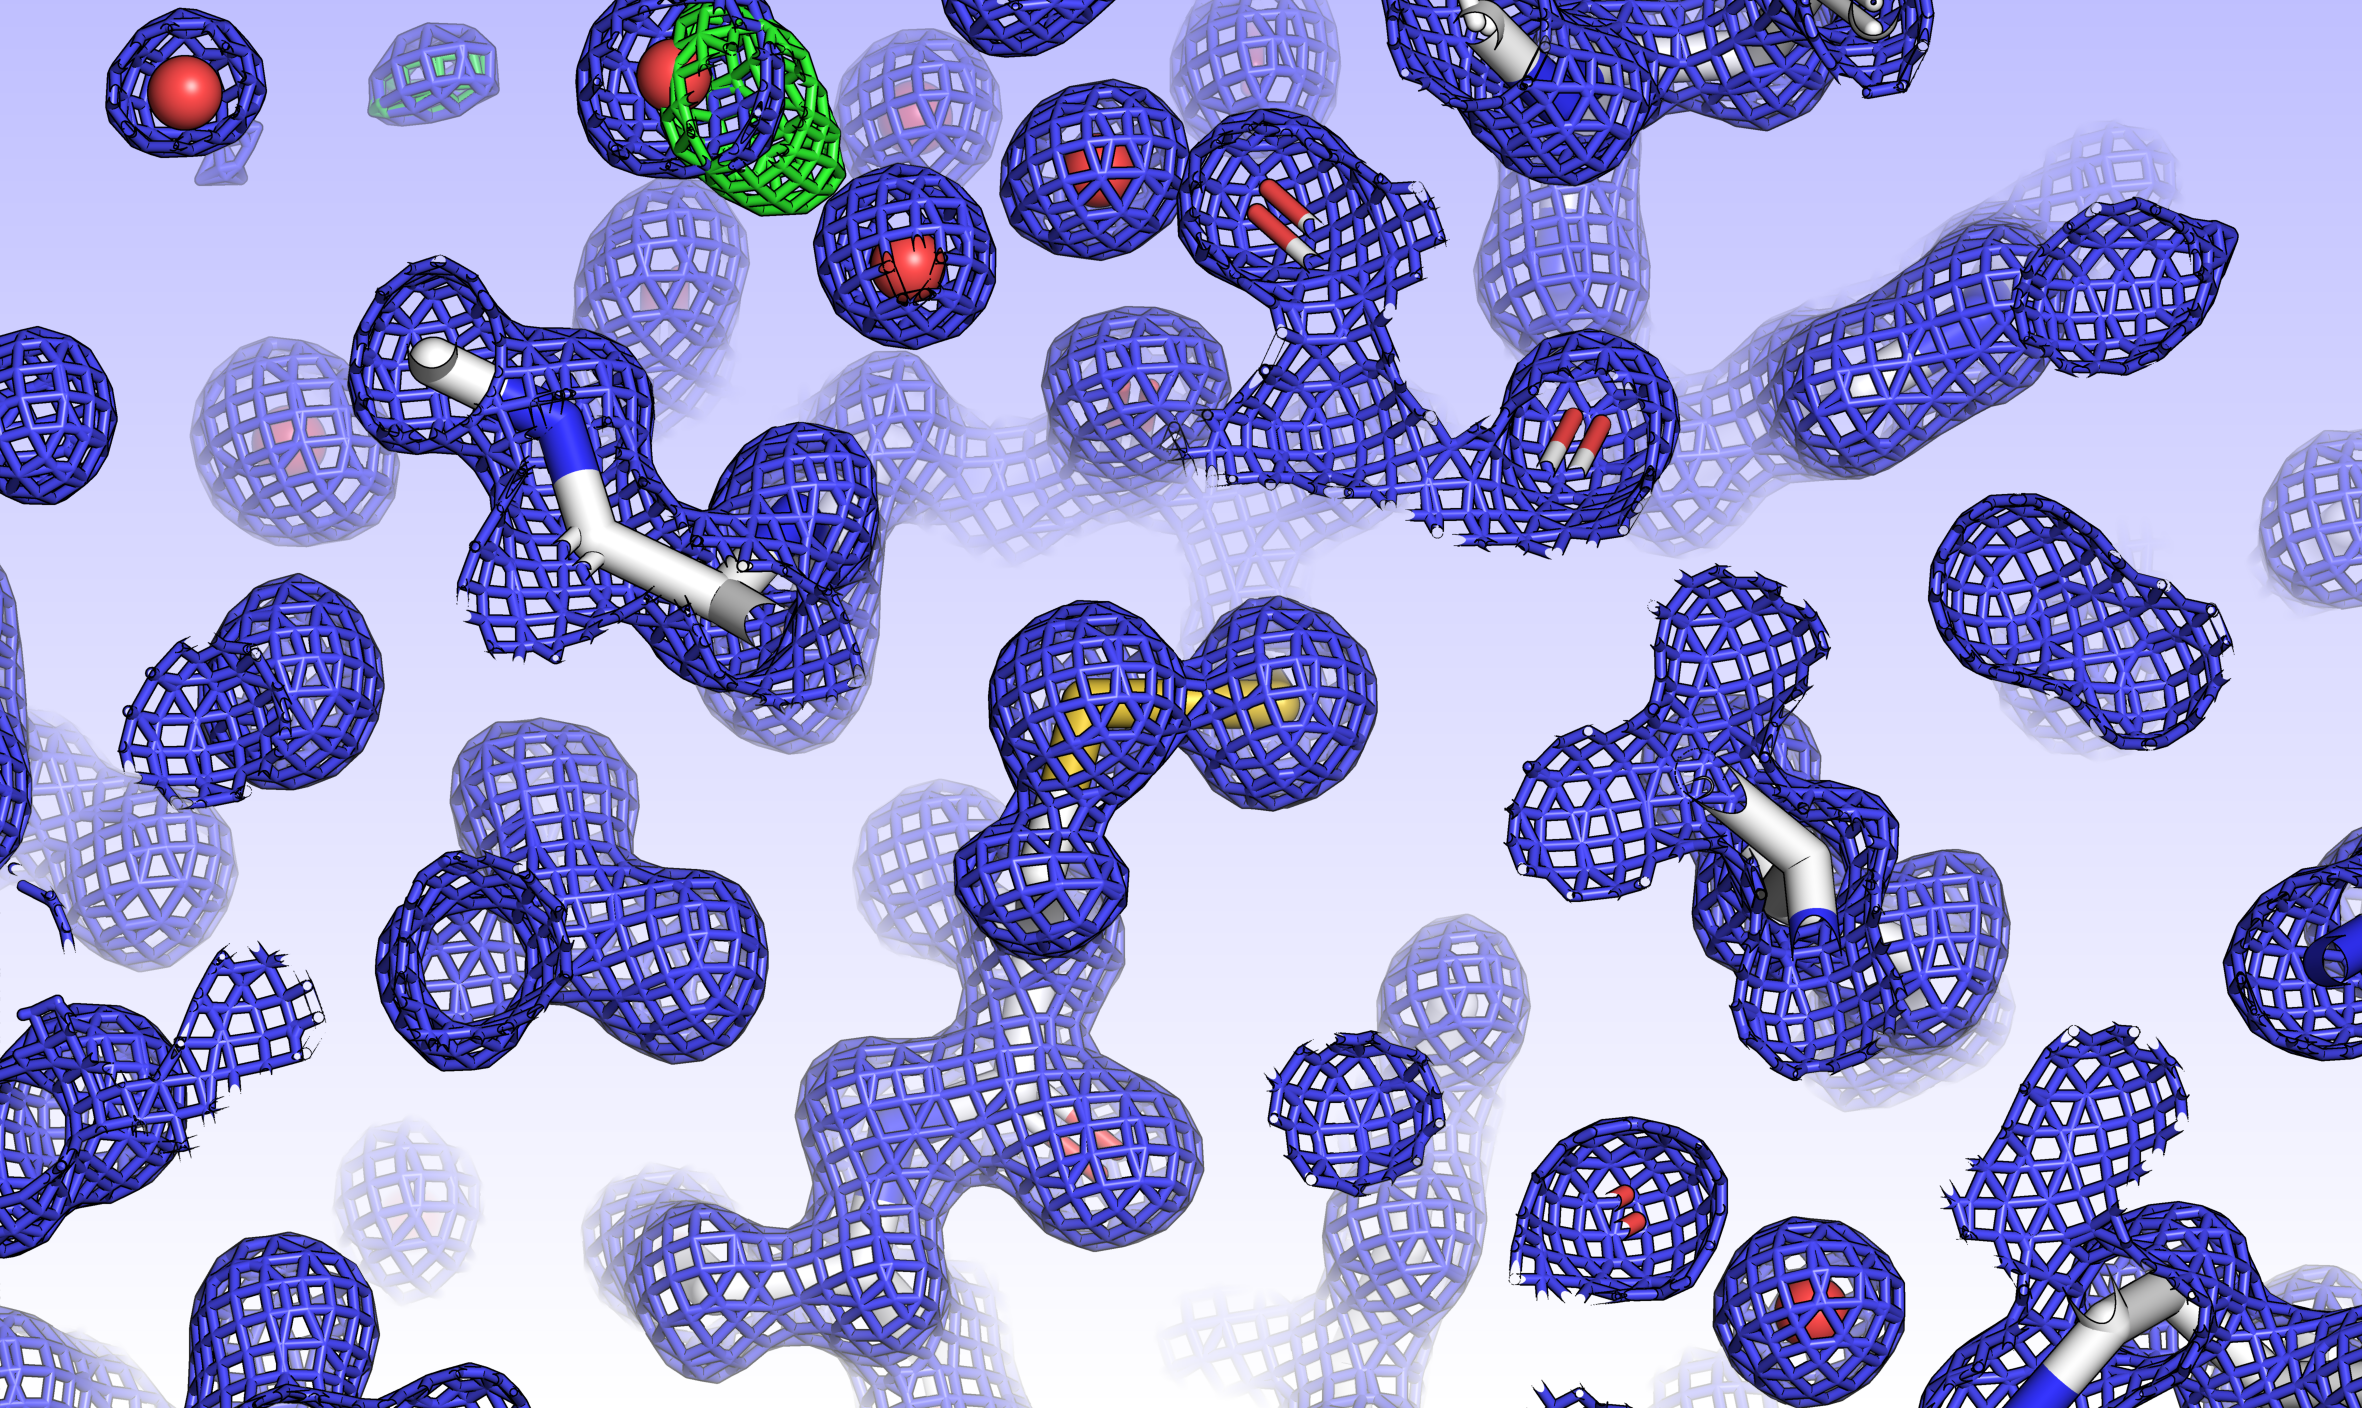
\includegraphics[width=0.75\textwidth]{imgs/before}
	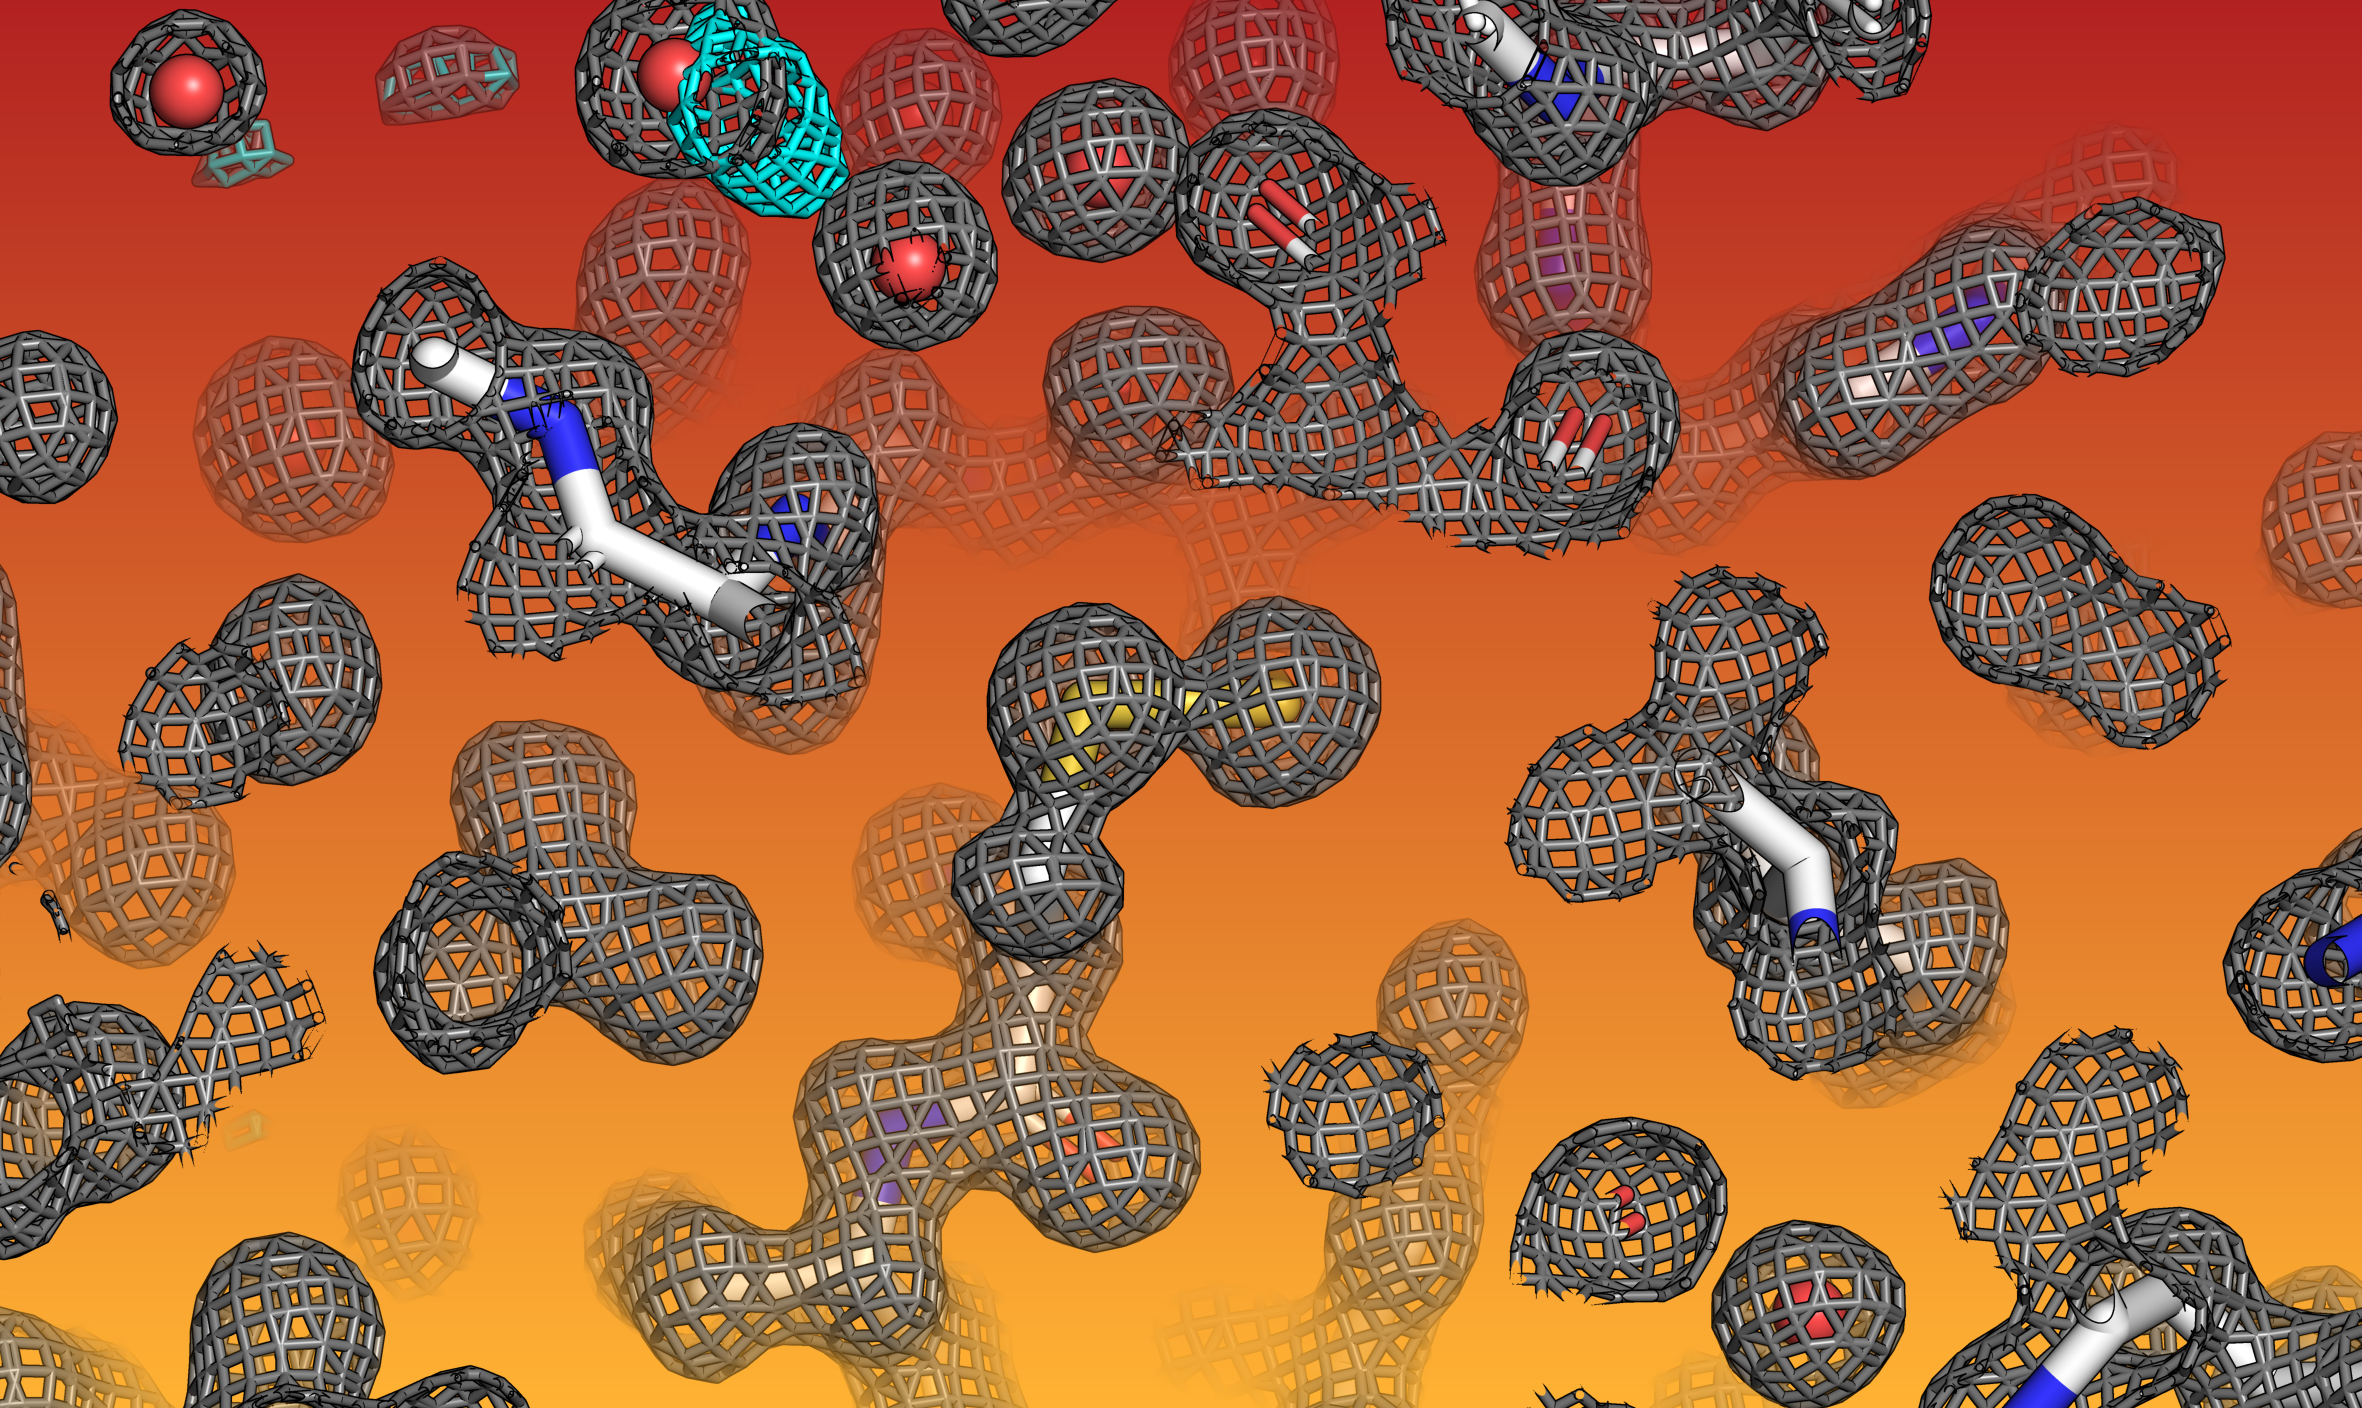
\includegraphics[width=0.75\textwidth]{imgs/after}
	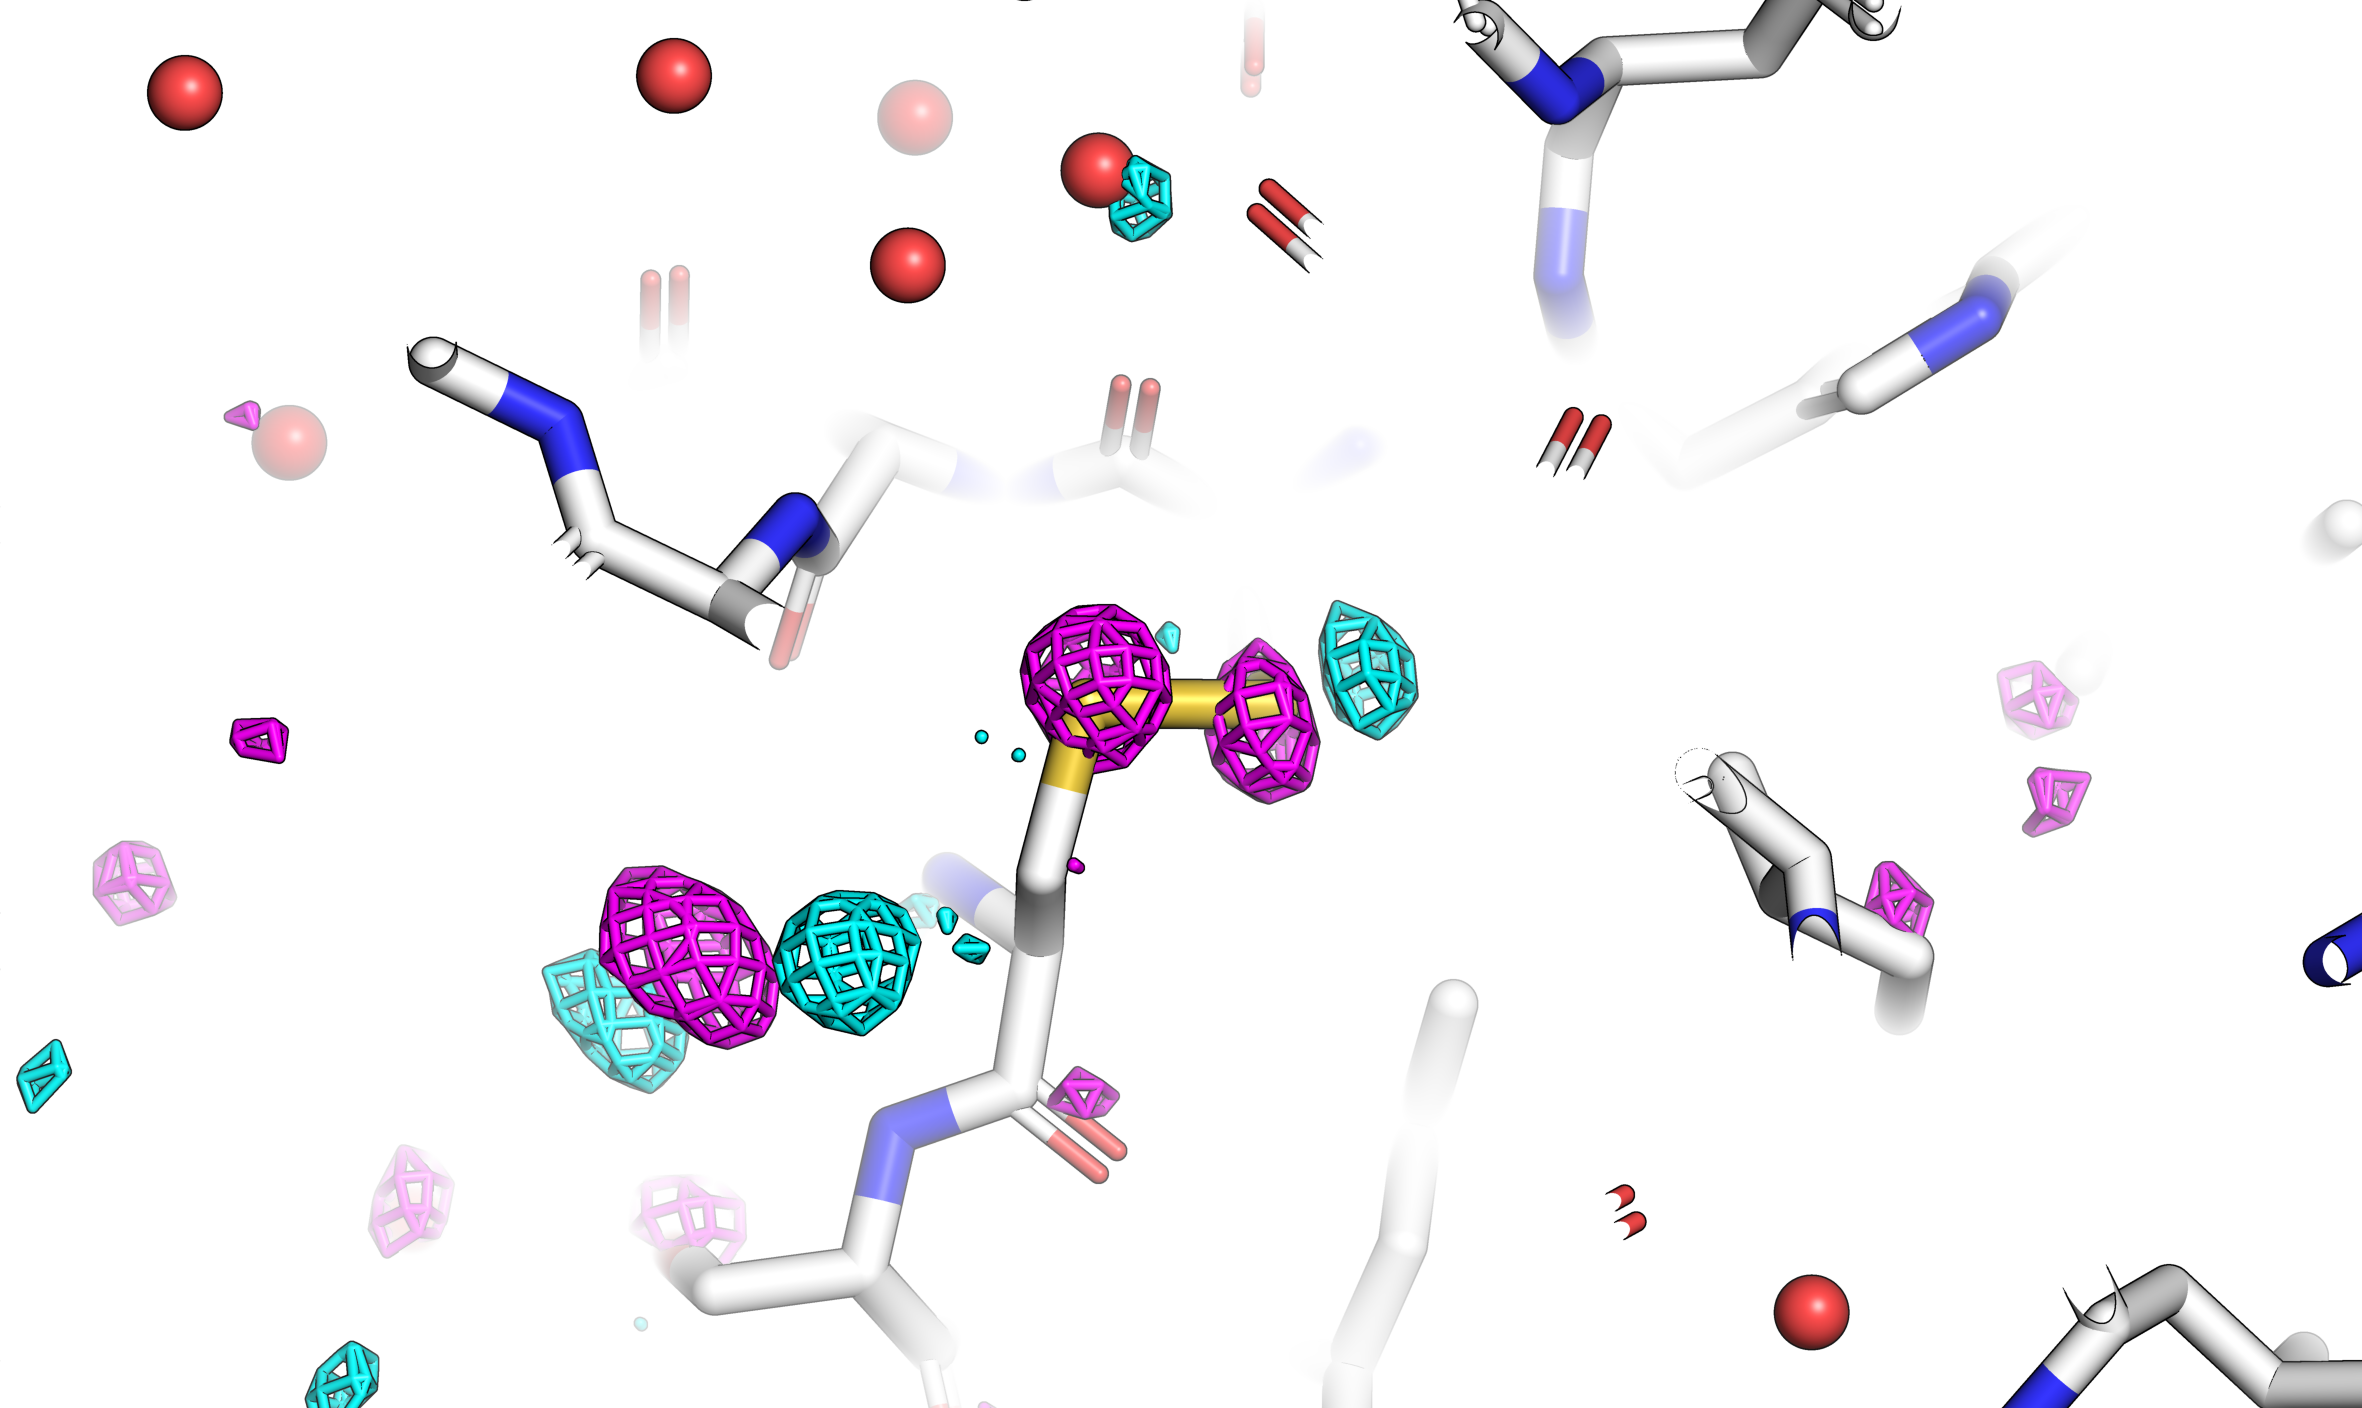
\includegraphics[width=0.75\textwidth]{imgs/diff}
	\caption[Diferencia de densidad electrónica]{Diferencia de densidad electrónica entre colectas de datos idénticas. Arriba: primer colecta de un cristal de lisozima (dosis absorbida \SI{0.6}{\mega\gray}). En medio: segunda colecta del mismo cristal (dosis absorbida \SI{3.2}{\mega\gray}). Los mapas $2F_{\mathrm{o}}-F_{\mathrm{c}}$ y $F_{\mathrm{o}}-F_{\mathrm{c}}$ se encuentran dibujados a \SI{1}{\sigma} y $\pm$\SI{3.5}{\sigma}, respectivamente. Abajo: La diferencia de densidad electrónica entre colectas $F_{\mathrm{o,2}}-F_{\mathrm{o,1}}$. Donde la diferencia negativa (magenta) está a \SI{-3.5}{\sigma} y la positiva (cian) a \SI{3.5}{\sigma}. Nótese como prácticamente no se observa una diferencia entre los mapas $2F_{\mathrm{o}}-F_{\mathrm{c}}$ (malla azul contra malla gris); sin embargo, sí existe una diferencia del modelo estructural inicial (el mismo en las tres imágenes) con respecto a la densidad electrónica de la segunda colecta. En otras palabras, para la segunda colecta, en una fracción de las proteínas cristalizadas este puente disulfuro se ha roto. Imagen realizada con PyMOL \cite{pymol} y datos de \cite{Nanao2005}. }
	\labfig{fig:difden}
\end{figure}


\section{Crioprotección}
\labsec{crio}
La primer estructura macromolecular determinada fue la de la mioglobina en 1958 por Kendrew y colaboradores \sidecite{Kendrew1958}. La forma de contender con el daño por radiación en aquella época era utilizando decenas de cristales y promediar los patrones de difracción. La regla de dedo para cambiar el cristal irradiado por uno nuevo, era seguir la intensidad de algunas reflexiones y si esta llegaba a disminuir de \num{20} a \SI{30}{\percent} de su valor inicial, entonces se procedía a reemplazar el cristal. 

El primer estudio en el que se valoró el potencial de la crioprotección, para reducir el daño por radiación, surgió por necesidad. Sucedía que ciertos cristales de insulina con átomos pesados sufrían un rápido desgaste por la radiación, en comparación con cristales de insulina sin átomos pesados. Con base en la observación de que el daño secundario es dependiente, en parte, de la temperatura; Low \emph{et al.} compararon, de manera cualitativa, el deterioro de los patrones de difracción colectados a \num{21}, \num{0} y a \SI{-13}{\celsius}. Los resultados fueron claros: a menor temperatura, mayor el tiempo de vida útil de los cristales  \sidecite{Low1966}. 

El problema con la reducción de temperatura en cristales macromoleculares, era la formación de hielo dentro de estos. Fue Haas quien primero usó crioprotectores para prevenir este problema. En el primer caso logró reducir la temperatura hasta \SI{-50}{\celsius}, remojando cristales de lisozima entrecruzados con glutaraldehído
en una mezcla de agua con glicerol \sidecite{Haas1968}. En un estudio posterior con cristales de lactato deshidrogenasa, el proceso de entrecruzamiento destruía los cristales. En cambio, si solo eran remojados por un par de días en una solución con sacarosa, el daño por radiación era diez veces menor \sidecite{Haas1970}. 
Es hasta 1988 que Hope describe por primera vez lo que conocemos hoy en día como criocristalografía de rayos X, donde básicamente se añade al cristal, o a la condición de cristalización, un crioprotector y el proceso de difracción del cristal se realiza a \SI{-173}{\celsius} \sidecite{Hope1988}. Una de las desventajas de esta técnica es encontrar las condiciones de crioprotección adecuadas para cada macromolécula. A pesar de este detalle, la crioprotección fue ganando adeptos de tal forma
que para el año 2000 era parte de la rutina de la \acrshort{drx} \sidecite{Garman2003}. Gracias a la crioprotección, en general era suficiente un único cristal macromolecular para obtener un
\enquote{dataset} completo.

\section{Sincrotrones}
\labsec{sincro}
La principales fuente de rayos X para realizar el experimento de \acrshort{drx}, es la radiación sincrotrón.
La historia tecnológica de los sincrotrones se divide en generaciones. La primera generación de sincrotrones eran aquellos pertenecientes al campo de la física de partículas, donde los primeros estudios con respecto a la estructura de proteínas fueron realizados \sidecite{Phillips1976}. Para la década de 1980 se construyen los sincrotrones dedicados a la biología estructural, esta es la segunda generación. Para la década de 1990 llega la tercera generación. El primer sincrotrón perteneciente a la cuarta generación empezó a operar en 2016 \sidecite{Owen2016}. 
Una de las características de un sincrotrón es su brillo espectral, que se define como la distribución del flujo de fotones en el espacio y el rango angular. El flujo se establece como el número de fotones por segundo que atraviesan un área definida por un ancho de banda dado \sidecite{Willmott2019}. La revolución tecnológica de los sincrotrones se nota en la diferencia del orden de magnitud del brillo espectral \cite{Willmott2019}. Este aumento en brillo se ha permitido pues permite una gran ventaja: la posibilidad de utilizar cristales de menor tamaño. Esto es porque la principal limitante de la \acrshort{drx} es obtener cristales macromoleculares, en particular cristales de un tamaño adecuado (al menos unos cien micrómetros en sus tres dimensiones\sidenote{Existen líneas especiales donde existe la posibilidad de usar cristales con un orden de magnitud menor, las denominadas líneas microfoco.}.) 

Actualmente se está desarrollando la tecnología para cambiar la metodología de la colecta de datos, usando cristales macromoleculares nanométricos y con una fuente de rayos X más poderosa denominada \acrshort{xfel} (del inglés \emph{X-ray Free Electron Laser}). Existen ya varios estudios en los que se ha demostrado la posibilidad de obtener estructuras macromoleculares con esta nueva metodología \sidecite{Martin-Garcia2016}. Sin embargo, el acceso al tiempo experimental en un XFEL es actualmente muy limitado.

Como se mencionó en la sección anterior, ya para el año 2000, la noción general en el campo de la criocristalografía era que el daño por radiación era insignificante, un problema del pasado. Precisamente esta noción cambia en ese mismo año, cuando tres estudios independientes muestran el efecto del daño por radiación en la entonces nueva generación de sincrotrones \sidecite{Teng2000,Weik2000,Ravelli2000}. 

\section{Radioprotectores}
\labsec{radio}
Al ser evidente que el daño por radiación aumentaba con el incremento en brillo, fue necesario buscar estrategias, como la crioprotección, que ayudaran a mitigar el daño por radiación. En el curso de los últimos veinte años, se han investigado varias estrategias pre y posteriores a la difracción con distintos enfoques \sidecite{Garman2017}. Una de las tantas estrategias, es el uso de moléculas pequeñas que interactuan con los radicales libres generados por la radiación. Estas moléculas se denominan radioprotectores. Sin embargo, en la literatura científica existen varias incongruencias con respecto a la efectividad de los radioprotectores y es por esto que la comunidad cristalográfica no ha adoptado al cien por ciento el uso de radioprotectores de manera rutinaria \sidecite{Nowak2009, Allan2013}.

\chapter{Antecedentes}
\labch{antec}
\section{pH}
\labsec{ph}
Una estrategia nueva, investigada en la tesis de maestría del presente autor%\sidenote{Disponible en el siguiente enlace \url{https://github.com/murpholinox/tesis\_maestria}}
, fue modificar el pH dentro de los cristales macromoleculares. Esta idea se basa en la idea general de los radioprotectores y se detalla a continuación. 

La radiólisis del agua produce las siguientes reacciones \sidecite{VonSonntag2006}:
\begin{align}
	\ce{H2O           &->[rayos X]     H2O^{.+}    +             e^{-}}  \\
	\ce{H2O           &->[rayos X]     H2O^{*}}                          \\
	\ce{H2O^{.+}      &->  \color{red}HO^{.}       +              H^{+}} \\
	\ce{e^{-} + nH2O  &->  \color{red}e^{-}_{solv.}}                     \\
	\ce{H2O^{*}       &->  \color{red}HO^{.}       +   \color{red}H^{.}}
\end{align} 
Donde las especies químicas denotadas en rojo, representan los primeros radicales libres presentes en un cristal macromolecular (el radical hidroxilo, el electrón solvatado y el radical hidrógeno).% Esto es relevante porque en general el contenido de solvente, agua, en un cristal macromolecular es bastante. 

Con la criocristalografía de rayos X, se impide la difusión del radical hidroxilo \sidecite{Owen2012a}. Sin embargo, el \ce{e^{-}_{solv.}} y el radical hidrógeno todavía son móviles. El electrón solvatado puede moverse del solvente a la proteína, donde es capaz de viajar a través de la cadena polipeptídica hasta hallar un centro electrofílico, como por ejemplo átomos metálicos o puentes disulfuro (\reffig{fig:symons92}) \sidecite{Symons1997}. Se ha propuesto que esta es la razón del origen del orden en el que se manifiesta el daño por radiación específico, pues la captura de electrones es mucho más específica que la captura de huecos positivos \sidecite{Close2019}. 

\begin{figure}[h]
	\centering
	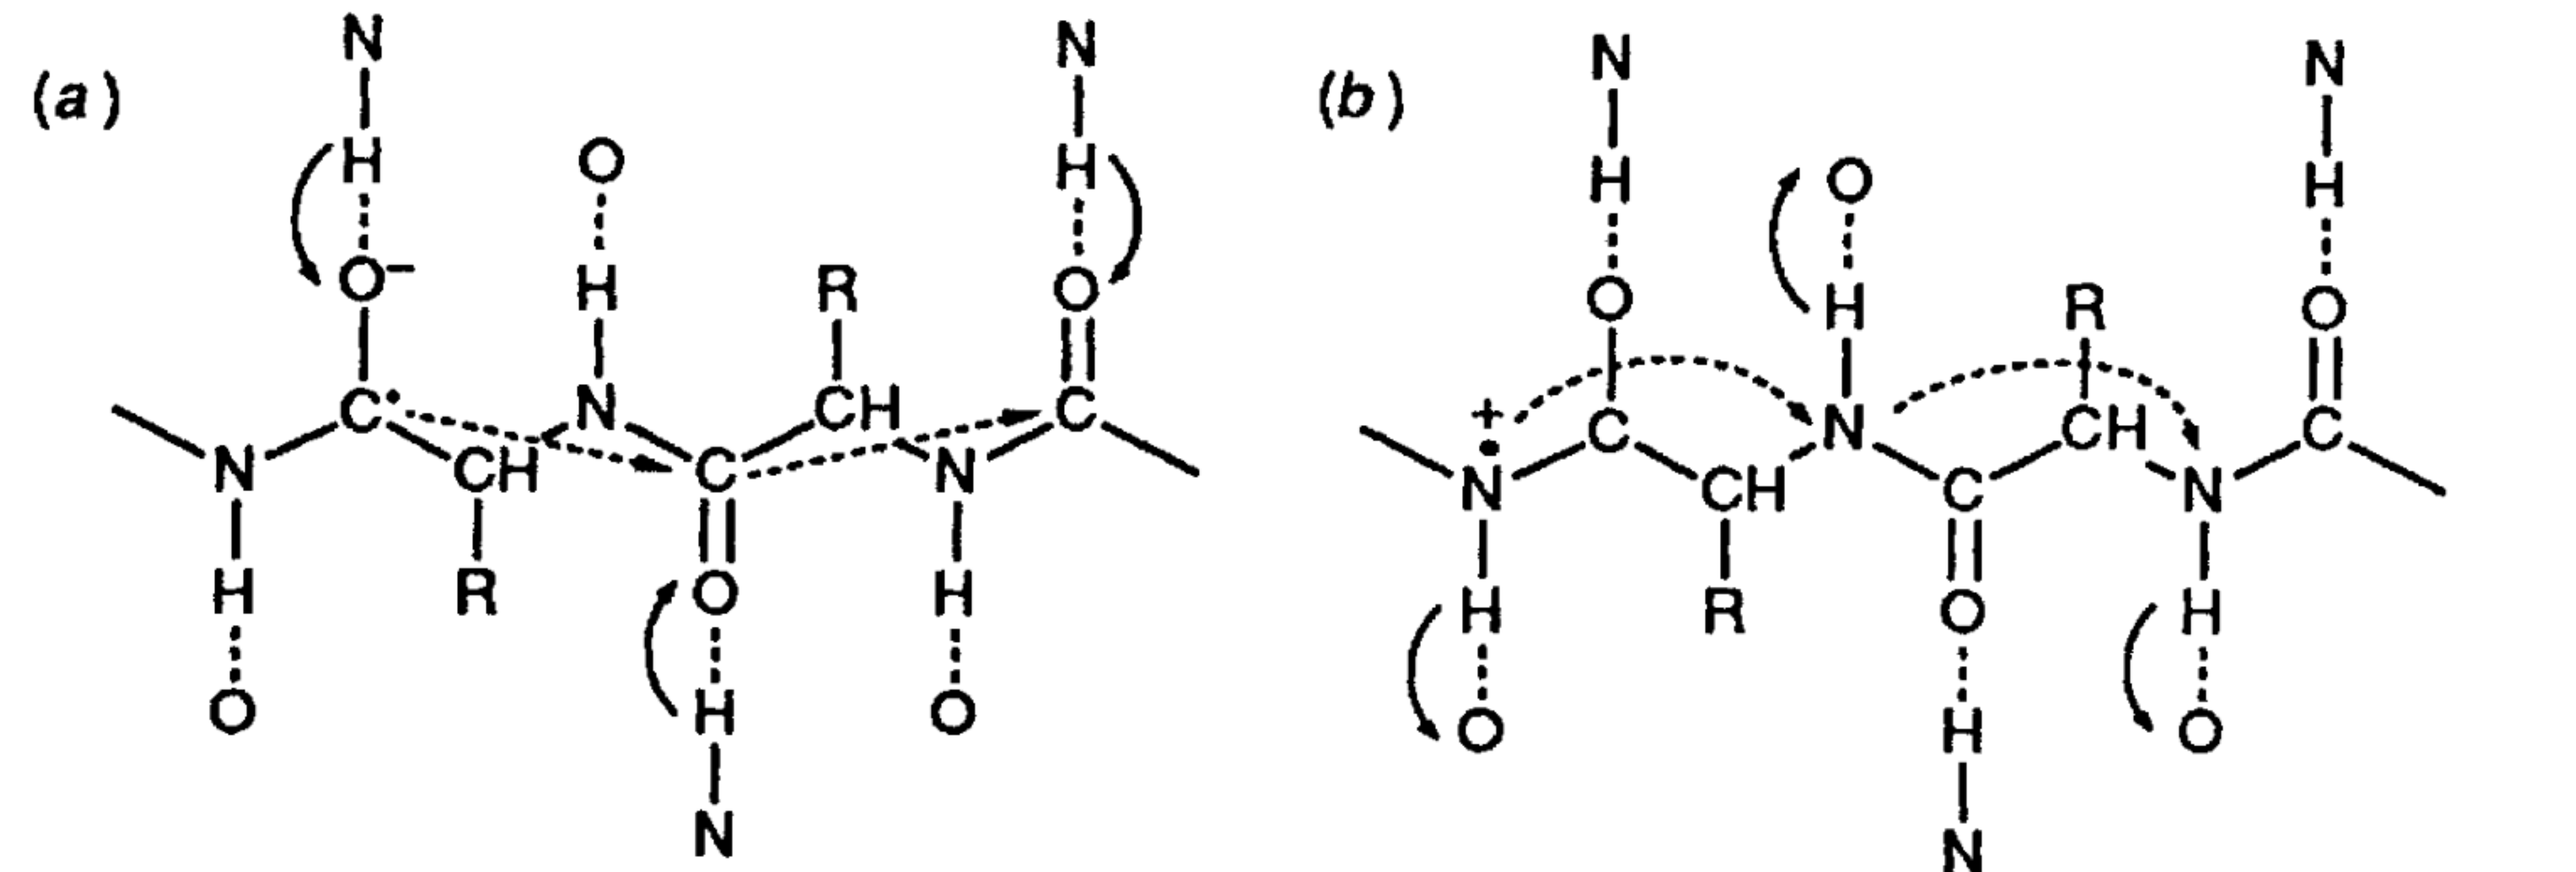
\includegraphics[width=0.9\textwidth]{imgs/symons92.png}
	\caption[Movimiento de cargas en la cadena polipeptídica]{Moviento de electrones (a) y huecos positivos (b), a través de la cadena polipeptídica. Fuente: \cite{Symons1997}.}
	\labfig{fig:symons92}
\end{figure}

Por su parte, el radical hidrógeno sigue una reacción de recombinación formando como producto final \ce{H2}, propuesto como el responsable directo del daño por radiación global \sidecite{Meents2010}.

La idea de ocupar al protón como radioprotector dentro del cristal macromolecular, se basa en que el electrón solvatado y el átomo de hidrógeno se encuentran en un equilibrio ácido-base; por lo que el electrón solvatado se convierte en \ce{H^{.}} en una solución ácida. %De hecho, en el campo de la química de las radiaciones, es común estudiar el efecto de un radical al convertir los otros radicales en especies el radical estudiado. 
\begin{equation}
\ce{e^{-}_{solv.} + H^{+} <=> H^{.}}
\end{equation}

En la tesis de maestría se usó como sistema de estudio la lisozima de clara de huevo de gallina, que presenta cuatro puentes disulfuro. La idea era que el ion hidronio, también conocido como oxidanio, funcionara como radioprotector al interactuar con los electrones solvatados antes que estos interactuaran con los puentes disulfuro de esta proteína. Para esto, se comparó el daño específico sobre los puentes disulfuro en cristales de lisozima a tres niveles de pH: \num{3.7}, \num{4.7} y \num{5.7}. Los resultados obtenidos fueron opuestos a los esperados: a niveles comparables de dosis de radiación absorbida, el cristal con el pH más ácido presentó mayor daño por radiación que el cristal con el pH más básico.

La variabilidad entre cristales macromoleculares, aún proveniendo de la misma condición de cristalización, puede llevar a conclusiones erróneas \sidecite{Nowak2009}. En la tesis de maestría no se pudo concluir si la diferencia observada era estadísticamente significativa, pues no se realizaron las repeticiones necesarias para cada condición experimental.



\chapter{Hipótesis}

La alta concentración de protones, es decir, bajos niveles de pH en la condición de cristalización, permitirán mitigar el daño por radiación en cristales de proteína. En particular el daño provocado por los \ce{e^{-}_{solv.}} y por lo menos a bajas dosis de radiación absorbida.
	

\chapter{Objetivo}
\labch{objet}

El objetivo de este proyecto es determinar el efecto del pH en la condición de cristalización de ciertas proteínas sobre el daño por radiación. 
\section{Objetivos particulares}
\labsec{objpar}
Para lograr el objetivo principal de este proyecto, se plantean los siguientes objetivos particulares:

Obtener mapas de diferencia de densidad electrónica entre puntos fijos de dosis de radiación absorbida.

\begin{enumerate}
	\item Realizar un análisis \emph{in silico} para determinar qué proteínas son capaces de cristalizar en un intervalo de pH amplio.
	\item Cristalizar las proteínas seleccionadas a diferentes niveles de pH usando cualquiera de los sistemas de amortiguamiento que muestrean un intervalo de pH amplio
	\item Determinar los parámetros de la colecta de datos que produzcan niveles similares o idénticos de dosis de radiación absorbida en las diferentes proteínas cristalizadas.
	\item Realizar colectas de datos continuas y seriales en un sincrotrón.
	\item Procesar los patrones de difracción para obtener un modelo inicial de las proteínas.
	\item Mapear la diferencia de densidad electrónica entre colectas de datos al modelo inicial de cada proteína y realizar un análisis comparativo, en particular sobre los residuos de aminoácido que son más susceptibles al daño por radiación, para determinar las diferencias en daño por radiación a diferentes niveles de pH.
\end{enumerate}	
\chapter{Materiales y métodos}
\labch{mayme}

\section{Proteínas seleccionadas}
El \acrshort{pdb} contiene información acerca de cientos de miles de proteínas cristalizadas en diferentes condiciones de cristalización. Para hallar qué proteínas pueden cristalizar en un amplio intervalo de pH se realizó un análisis \emph{in silico}, como se explica brevemente\sidenote{Con detalle en \url{https://github.com/murpholinox/doctorado}.} a continuación. 

\subsection{Extracción de datos}
%\sidenote{Actualmente la API fue reemplazada por una nueva versión cuyo desarrollo no ha sido completado \url{https://tinyurl.com/y84kuvs7}.}
Se extrajo la información experimental directamente del cabezal de los archivos de las estructuras depositadas en el \acrshort{pdb}. Para extraer la información de los cabezales se usó el programa \Package{gemmi}\sidenote{Disponible en el siguiente enlace \url{https://github.com/project-gemmi/gemmi}.}. La información extraída es la siguiente: el contador de la entidad macromolecular, el tipo de entidad, el código de acceso de la base de datos de referencia\sidenote{La mayoría de las veces el código usado es aquél de la base de datos UniProt \url{https://www.uniprot.org/}.}, su descripción, el método experimental para crecer los cristales, el pH de la condición de cristalización, los detalles del experimento de la cristalización, la resolución final del modelo estructural, el grupo espacial en el que cristaliza la macromolécula y el identificador de objeto digital de la publicación científica correspondiente. A continuación se muestra un ejemplo de la información extraída:

\begin{kaobox}[frametitle=Ejemplo 1]
\begin{verbatim}
6LU7,1,polypeptide(L),P0DTD1,main protease,EVAPORATION,\
6,"2% polyethylene glycol (PEG) 6000, 3% DMSO, 1mM DTT,\
0.1M MES buffer (pH 6.0), protein concentration 5mg/ml,\
VAPOR DIFFUSION, HANGING DROP, temperature 293K",2.16,\
2.16,C 1 2 1,10.1038/s41586-020-2223-y,21728,210031
6LU7,2,polypeptide(L),P0DTD1,main protease,EVAPORATION,\
6,"2% polyethylene glycol (PEG) 6000, 3% DMSO, 1mM DTT,\
0.1M MES buffer (pH 6.0), protein concentration 5mg/ml,\
VAPOR DIFFUSION, HANGING DROP, temperature 293K",2.16,\
2.16,C 1 2 1,10.1038/s41586-020-2223-y,21728,210031
\end{verbatim}
\end{kaobox}

El resultado final es una tabla de datos, con \num{226523} observaciones, o filas, y \num{14} variables, o columnas. El número de observaciones es mayor que el número de estructuras depositadas en el \acrshort{pdb} y esto es debido a que cada entrada puede tener más de una macromolécula, como se puede notar en el \Environment{Ejemplo 1}. La integridad de los datos se puede verificar al graficar algunas de las variables extraídas.

\subsection{Limpieza de datos}
Se aplican los siguientes filtros a los datos extraídos para eliminar observaciones que:

\begin{enumerate}
	\item Carecen de un código de acceso.
	\item Tienen una resolución peor que \SI{2}{\angstrom}. 
	\item Carecen del valor de pH de la condición de cristalización.
	\item El número de entidades es mayor o igual a dos.
\end{enumerate}

La lógica de los filtros es la siguiente: (\emph{i} y \emph{iii}) Remover entradas que no tengan las anotaciones correspondientes\sidenote{Desafortunadamente, la información experimental no siempre se encuentra en los archivos del PDB.}, en este caso el código de acceso de la proteína y el pH de la condición de cristalización. Siendo la última la anotación más relevante para este proyecto y la primera, es la única manera de conocer casi inequívocamente la proteína representada en el archivo. (\emph{ii}) La resolución final del modelo estructural es un indicador \emph{grosso modo}, de la calidad del cristal obtenido. Este filtro garantiza que el listado de proteínas obtenidas sean fáciles de cristalizar. Además este filtro sirve para el análisis posterior, al comparar el daño por radiación específico entre proteínas/pHs, pues los resultados serán más confiables con una buena resolución. (\emph{iv}) Como se mencionó anteriormente, un archivo puede contener múltiples macromoléculas. Este filtro ayuda a descartar proteínas cristalizadas con otras. En general, las condiciones de cristalización para combinaciones diferentes de macromoléculas serán diferentes; por lo que no tiene caso tener varias observaciones de la misma proteína, si esta cristaliza con diferentes macromoléculas. 

En el apéndice se listan las 50 proteínas más representadas en el \acrshort{pdb}, cuando cumplen los primeros cuatro filtros (\reftab{tab:top50}). 

Posteriormente se aplican los siguientes dos filtros, que ayudan a eliminar las observaciones donde:

\begin{enumerate}
	\setcounter{enumi}{4}
	\item Su secuencia de aminoácidos sea diferente de la secuencia consenso para cada conjunto de proteínas.
	\item No presenten un intervalo de pH amplio en su cristalización.
\end{enumerate}

La lógica de estos dos filtros es la siguiente: (\emph{v}) elimina entradas donde el número de mutaciones, sustituciones o deleciones, sea mayor o igual a quince. Esto elimina, por ejemplo, aquellas proteínas cristalizadas con el péptido señal (en caso de tenerlo) y, por otra parte, mantiene entradas de aquellas proteínas cristalizadas con etiquetas de purificación por afinidad (siempre y cuando la etiqueta no sea mayor de quince péptidos).  Además elimina entradas donde la secuencia de la proteína, no corresponda a la secuencia consenso. En general, cada proteína tiene uno o varios identificadores UniProt. En el caso de las poliproteínas de algunos virus, el identificador de la poliproteína es el mismo para las subproteínas. A continuación se muestra un ejemplo:

\begin{kaobox}[frametitle=Ejemplo 2]
	\begin{verbatim}
	6W4H,1,polypeptide(L),P0DTD1,SARS-CoV-2 NSP16,...
	6W4H,2,polypeptide(L),P0DTD1,SARS-CoV-2 NSP16,...
	6W6Y,1,polypeptide(L),P0DTD1,SARS-CoV-2 NSP3,...
	6WQD,1,polypeptide(L),P0DTD1,SARS-CoV-2 NSP7,...
	6WQD,2,polypeptide(L),P0DTD1,SARS-CoV-2 NSP7,...
	7BUY,1,polypeptide(L),7BUY,SARS-CoV-2 virus Main protease,
	\end{verbatim}
\end{kaobox}


Es claro que el código, \texttt{P0DTD1}, es el mismo; sin embargo, las observaciones corresponden a diferentes proteínas.

El alineamiento múltiple se realizó con el programa \Package{mafft} \sidecite{Katoh2013}. La secuencia consenso se obtuvo con el programa \Package{cons} de la suite de programas \Package{emboss} \sidecite{Madeira2019}. Para la determinación del número de mutaciones se aplicó la función \Package{adist} \sidenote{\url{https://www.rdocumentation.org/packages/utils/versions/3.6.2/topics/adist}} en el lenguaje de programación \Package{R}. 

Y, (\emph{vi}), es la condición experimental que nos interesa en este proyecto, proteínas que cristalicen en un amplio intervalo de pH. Este filtro se aplicó por partes. Primero se realizó un gráfico de caja para cada una de las 50 proteínas más representadas en los datos. Este tipo de gráfica da una representación visual de la distribución de la variable en cuestión. Si la distribución no cubre al menos tres unidades de pH, entonces se descarta dicha proteína, en caso contrario se mantiene. De las proteínas restantes, 25, se realiza un histograma de frecuencias para determinar de manera cuantitativa la frecuencia con la que cada proteína ha sido cristalizada en valores de pH diferentes. Si la frecuencia no es mayor a cinco para la mayoría de las barras en cada histograma, la proteína se descarta, si no se mantiene. Esto resulta en un listado de 14 proteínas, donde las diez primeras entradas se presentan en la correspondiente sección de resultados (\reftab{tab:list}). 

\section{Cristalización de proteínas}
\subsection{Lisozima}
La lisozima de clara de huevo de gallina (\emph{Gallus gallus}), se obtuvo de manera comercial de \Package{Sigma-Aldrich}, con el número de catálogo \Package{L6876} de manera liofilizada. Según la hoja de datos tiene una pureza mayor o igual al \SI{90}{\percent} y por lo tanto no se realizó ningún paso de purificación subsecuente.

\subsection{Tripsina}
La tripsina pancreática de bovino (\emph{Bos taurus}), también se obtuvo de manera comercial de \Package{Sigma-Aldrich}, con el número de catálogo \Package{T4799} de manera liofilizada.\todo{Cuál es la pureza?} Tampoco se realizó ningún paso de purificación subsecuente.

\subsection{Amortiguadores de capacidad extendida}
De los sistemas de amortiguadores de capacidad extendida desarrollados por Newman \cite{Newman2004}, se utilizó la primera condición de cristalización (denominada de ahora en adelante, S1): ácido succínico, glicina y sodio dihidrógeno fosfato monohidratado a una concentración de \SI{250}{\milli\Molar}. \todo{Y posiblemente más!}

\subsection{Experimentos de cristalización}
Los experimentos de cristalización se realizaron con la técnica modificada de \emph{microbatch}, propuesta por D'Arcy \emph{et al.} \cite{DArcy1996}. 

En estos experimentos, se varió la concentración de la proteína (15 o \SI{30}{\milli\gram\per\milli\liter}); la proporción entre aceites de parafina y silicona (1:0, 1:0.5, 1:1, 1:2 y 1:4); el pH (10, 9.5, 9.0, $\ldots$, 4.5) y finalmente, también se cambió el porcentaje de cloruro de sodio (0, 3 y \SI{6}{\percent} p/v) en la condición de cristalización. Esto debido a que, en ciertas condiciones, se ha observado una dependencia del tamaño de los cristales de lisozima obtenidos con respecto a la concentración de cloruro de sodio \cite{Svanidze2005}. Se usaron placas de cristalización de Terasaki Greiner de \num{72} pozos. Esto permite tres corridas de pH, con tres porcentajes de cloruro de sodio por duplicado. Cabe destacar que en cada placa la proporción de aceites es diferente. 

\subsection{Clasificación de resultados de cristalizacion}
Para clasificar los resultados de cristalización, se usó un esquema de clasificación modificado a partir del esquema de Bruno \emph{et al.} \cite{Bruno2018}. La clasifiación es la siguiente: 1 (cristales), 0.5 (cristales pequeños), 0 (gota clara), -1 (precipitado) y -2 (otros). Se tomaron cuatro fotos con una cámara USB acoplada a un microscopio óptico en los días quinto, noveno, décimosexto y trigésimo octavo.

\section{Colecta y análisis de datos}
Los cristales obtenidos serán difractados en un sincrotrón. Para cada cristal macromolecular se tendrán que realizar series de colectas de datos de manera repetitiva. Gracias a la presencia de modelos estructurales en el \acrshort{pdb}, se puede estimar la dosis absorbida por la proteína antes de realizar el experimento de difracción. Esto se realiza gracias al programa \Package{raddose} \sidecite{Zeldin2013}. Se resolveran las estructuras por reemplazo molecular y se crearán mapas de diferencia de densidad electrónica para analizar la diferencia en daño por radiación específico a distintos pHs al mismo nivel de dosis de radiación absorbida. %Cabe señalar que la mayor parte del análisis posterior a la colecta de datos será \emph{in silico} y gracias al trabajo anterior se dispone de un flujo de trabajo semiautomático lo que facilitará en gran medida el presente proyecto.
\todo{Aquí obviamente falta poner los parámetros experimentales de las colectas de datos. }

\chapter{Resultados}

\section{Proteínas seleccionadas} 

Del análisis \emph{in silico} para determinar qué proteínas son capaces de cristalizar en un intervalo de pH amplio, se obtuvieron diez proteínas.

\begin{table}[h]
	\centering
	\begin{tabular}{@{}llll@{}}
		\toprule
		Número & Código & Intervalo       & Nombre                              \\ \midrule
		1      & P00918 & 6               & Anhidrasa carbónica                 \\
		2      & P00698 & 5.5             & Lisozima                            \\
		3      & P00760 & 6               & Tripsina                            \\
		4      & P02766 & 5               & Transtiretina                       \\
		5      & P42212 & 6               & Proteína verde fluorescente         \\
		6      & O60885 & 3.5             & Proteína bromodominio 4             \\
		7      & P19491 & 4.5             & Receptor de glutamato 2             \\
		8      & O26232 & 4               & Orotidina-5’-fosfato descarboxilasa \\
		9      & P00772 & 4.5             & Elastasa                            \\
		10     & P00644 & 3               & Termonucleasa                       \\
		\bottomrule
	\end{tabular}
	\caption[Proteínas que cristalizan en un intervalo amplio de pH]{Proteínas que cristalizan en un intervalo amplio de pH.}
	\labtab{tab:list}
\end{table}


\section{Cristalización}
Con la variación de parámetros experimentales para la cristalización, se obtuvieron \num{360} experimentos (\num{720}, tomando en cuenta los duplicados), por proteína. %Esto último, tiene que ver con la reproducibilidad de los resultados de los experimentos de cristalización, pues no siempre son idénticos.

\subsection{Lisozima}
Esto significa que se visualizaron y clasificaron \num{5760} fotos. Los resultados se definieron como positivos si se presentan cristales, en al menos uno de los dos experimentos, en los siguientes valores de pH 10, 9, 7.5, 5.0 y 4.5; de lo contrario, se consideran como resultados negativos. 
Los resultados positivos para la lisozima se resumen a continuación.


\begin{table}[h]
	\centering
	\begin{tabular}{@{}llll@{}}
		\toprule
		Proteína & Concentración & \% p/v NaCl & AP:AS \\ \midrule
		Lisozima & 15 & 3 & 1:1 \\
		Lisozima & 15 & 3 & 1:4 \\
		Lisozima & 15 & 6 & 1:4 \\
		Lisozima & 30 & 3 & 1:1 \\
		Lisozima & 30 & 6 & 1:1 \\
		Lisozima & 30 & 3 & 1:2 \\
		Lisozima & 30 & 6 & 1:2 \\
		Lisozima & 30 & 3 & 1:4 \\
		Lisozima & 30 & 6 & 1:4 \\ \bottomrule
	\end{tabular}
	\caption{Condiciones de cristalización exitosas para la lisozima. AP y AS significan aceite de parafina y silicona, respectivamente.}
	\label{tab:my-table}
\end{table}


\subsection{Tripsina}
Para la tripsina, por lo menos al momento del día de la tercera foto, todos los resultados fueron negativos. 

\section{Dosis de radiación}
Se escribió un programa en el lenguaje de programación \verb|bash| que permite obtener la dosis de radiación absorbida,  calculada por \verb|raddose| \cite{Bury2018}. Por simplicidad, se determinó un cristal hipotético de lisozima cúbico, con un volumen de \SI{1000000}{\cubic\angstrom}. Este presenta la misma composición atómica que la entrada \verb|1iee| del \verb|PDB|. También por simplicidad, el haz de rayos X se definió como colimado, con un corte de \num{100} x  \SI{100}{\micro\meter}, abarcando el área completa del cristal y un tiempo total de exposición de \SI{100}{\second}, con la obtención de un patrón de difracción por segundo. Dicho programa muestrea un flujo de fotones de 1.0 a \SI{100e11}{fotones\per\second} con un paso d \SI{0.1}{fotones\per\second} y una energía de 10.0 a \SI{17.2}{\kilo\electronvolt} con un paso de \SI{0.2}{\kilo\electronvolt}. Se obtuvo acceso al clúster \verb|groc| del grupo de genómica computacional del Instituto de Biotecnología de la UNAM\footnote{\url{https://biocomputo.ibt.unam.mx/}.}para correr dicho programa. Cabe aclarar que si bien los parámetros experimentales dados son idóneos, el fin de este programa es tener un estimado de la dosis por radiación absorbida en un sincrotrón de tercera generacion. Por otra parte, este primer programa sienta las bases para cualquier programa posterior en el que se necesite adaptar los parámetros experimentales a la realidad.

\section{Colectas de datos} 
%Con respecto a las colectas de datos, como primer acercamiento, se llevaron cinco\footnote{Crecidos a pH 10 (dos), 7.5 (uno) y 4.5 (dos).} cristales de lisozima al Laboratorio Nacional de Estructura de Macromoléculas (LANEM) del Instituto de Química (IQ) de la UNAM el 20 de mayo del presente año. En el LANEM-IQ, se tiene acceso a un generador de rayos X \verb|MicroMax-007 HF| de \verb|Rigaku|\footnote{\url{https://www.rigaku.com/products/sources/mm007}}. Hasta el momento, el único dato del que se tiene conocimiento es que la difracción de al menos uno de los cristales era mejor que \SI{1.6}{\angstrom}. 


%\pagelayout{wide} % No margins
%\addpart{Title of the Part}
%\pagelayout{margin} % Restore margins

\appendix % From here onwards, chapters are numbered with letters, as is the appendix convention

\chapter{Proteínas más representadas}
\labch{top50}

Se listan las 50 proteínas más representadas en el \acrshort{pdb}, cuando cumplen los primeros cuatro filtros, mencionados en la sección: Limpieza de datos.

\begin{table}[h]
	\centering
	\begin{tabular}{@{}llllll@{}}
	\toprule
	Número & Código    & Entradas & No. & Código       & Entradas \\* \midrule

1      & \texttt{P11838} & 689    & 26     & \texttt{P23497}     & 106  \\
2      & \texttt{P00918} & 619    & 27     & \texttt{P00800}     & 103  \\
3      & \texttt{P00698} & 498    & 28     & \texttt{O26232}     & 102  \\
4      & \texttt{P00760} & 310    & 29     & \texttt{P22629}     & 97   \\
5      & \texttt{Q6PJP8} & 296    & 30     & \texttt{P00489}     & 96   \\
6      & \texttt{Q6B0I6} & 269    & 31     & \texttt{P03367}     & 96   \\
7      & \texttt{P02766} & 258    & 32     & \texttt{P68400}     & 95   \\
8      & \texttt{O95696} & 257    & 33     & \texttt{A0A073FPA6} & 84   \\
9      & \texttt{Q9UIF8} & 227    & 34     & \texttt{P46881}     & 79   \\
10     & \texttt{P00644} & 216    & 35     & \texttt{P00811}     & 78   \\
11     & \texttt{P00720} & 215    & 36     & \texttt{Q16539}     & 77   \\
12     & \texttt{P24941} & 203    & 37     & \texttt{P14174}     & 75   \\
13     & \texttt{P42212} & 182    & 38     & \texttt{P00431}     & 73   \\
14     & \texttt{P29476} & 178    & 39     & \texttt{P01116}     & 73   \\
15     & \texttt{P02185} & 172    & 40     & \texttt{P00183}     & 72   \\
16     & \texttt{O60885} & 170    & 41     & \texttt{P01112}     & 72   \\
17     & \texttt{P18031} & 152    & 42     & \texttt{Q00511}     & 70   \\
18     & \texttt{P61823} & 145    & 43     & \texttt{Q76353}     & 68   \\
19     & \texttt{P28720} & 144    & 44     & \texttt{P00282}     & 64   \\
20     & \texttt{P07900} & 142    & 45     & \texttt{P02883}     & 63   \\
21     & \texttt{P61626} & 139    & 46     & \texttt{P02945}     & 63   \\
22     & \texttt{P15121} & 125    & 47     & \texttt{P06873}     & 63   \\
23     & \texttt{P56817} & 124    & 48     & \texttt{P16113}     & 63   \\
24     & \texttt{P0DTD1} & 123    & 49     & \texttt{Q04609}     & 63   \\
25     & \texttt{P19491} & 116    & 50     & \texttt{P00772}     & 61   \\ \bottomrule
	\caption[Las 50 proteínas más representadas]{Las 50 proteínas más representadas en los datos, después de los cuatro primeros filtros. Eliminando estructuras que no contienen: código de acceso ni el valor de pH de la condición experimental. Además descarta aquellas estructuras con una resolución peor que \SI{2}{\angstrom} y donde el número de entidades es mayor o igual a dos.}
	\labtab{tab:top50}
	\end{tabular}
\end{table}


%\chapter{Análisis visual}
\labch{vis-anal}
\begin{figure}[h!]
	\centering
	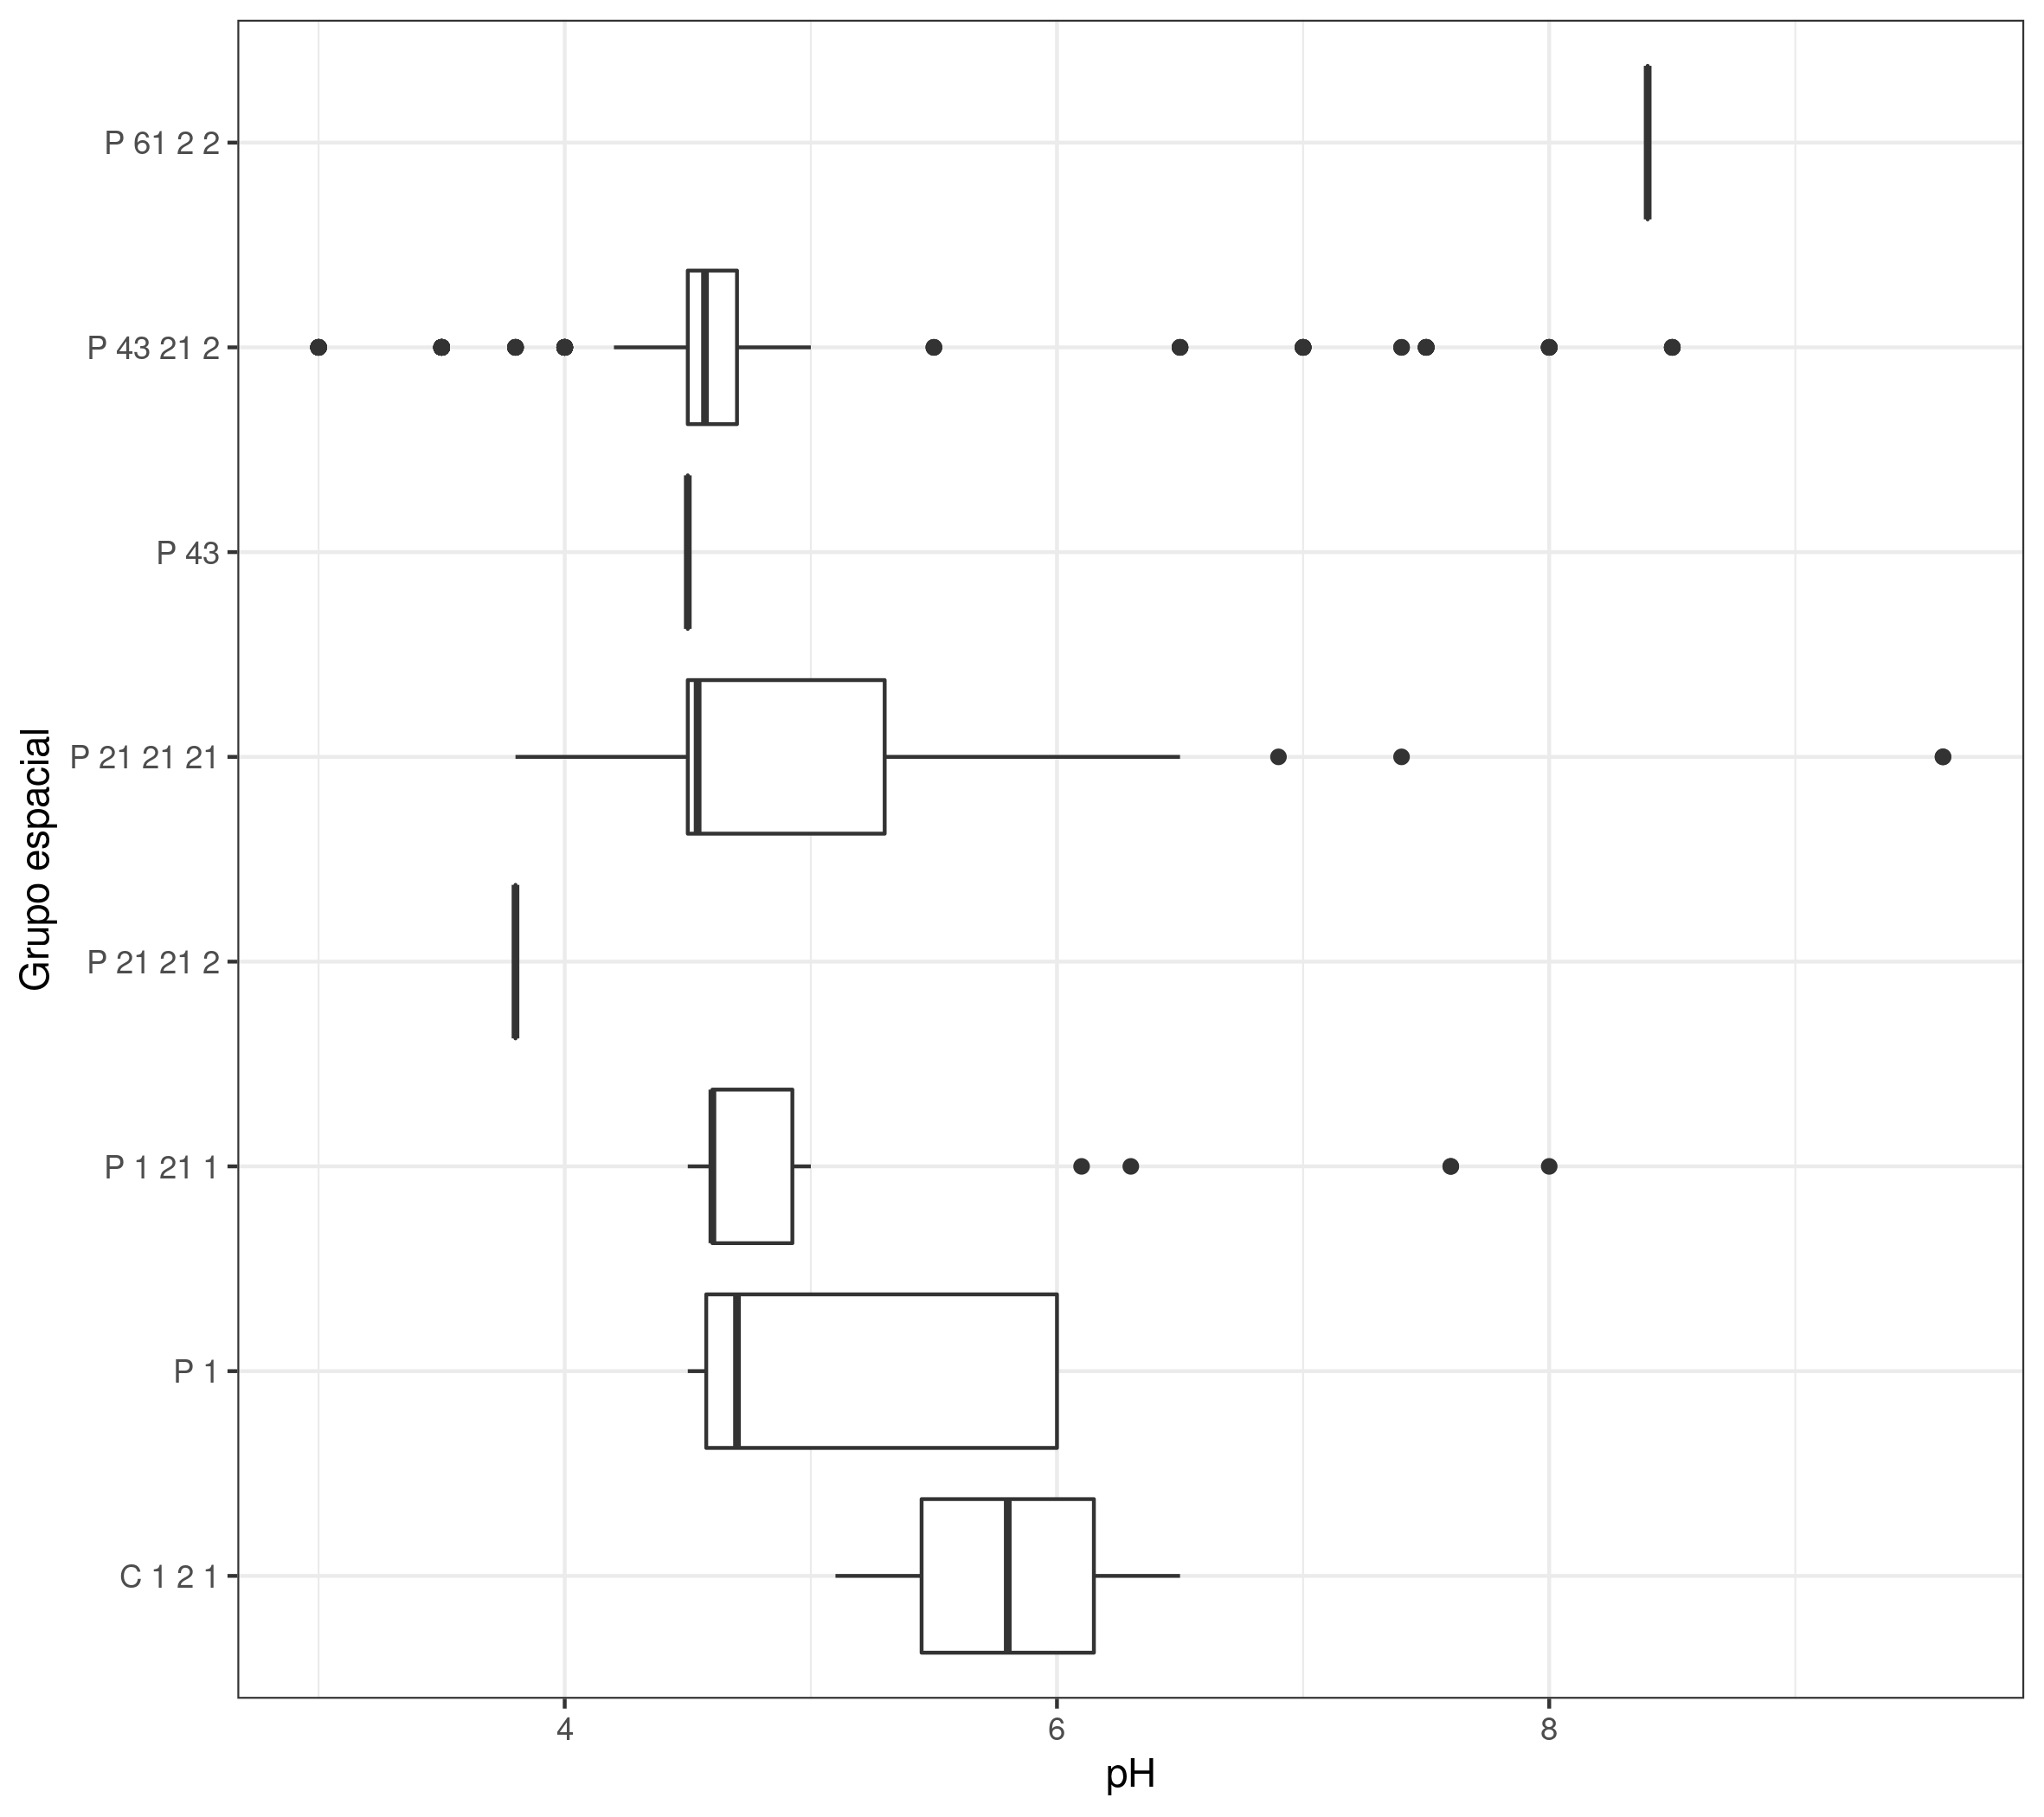
\includegraphics[width=0.8\textwidth]{imgs/box_pH_by_gpo_P00698}
	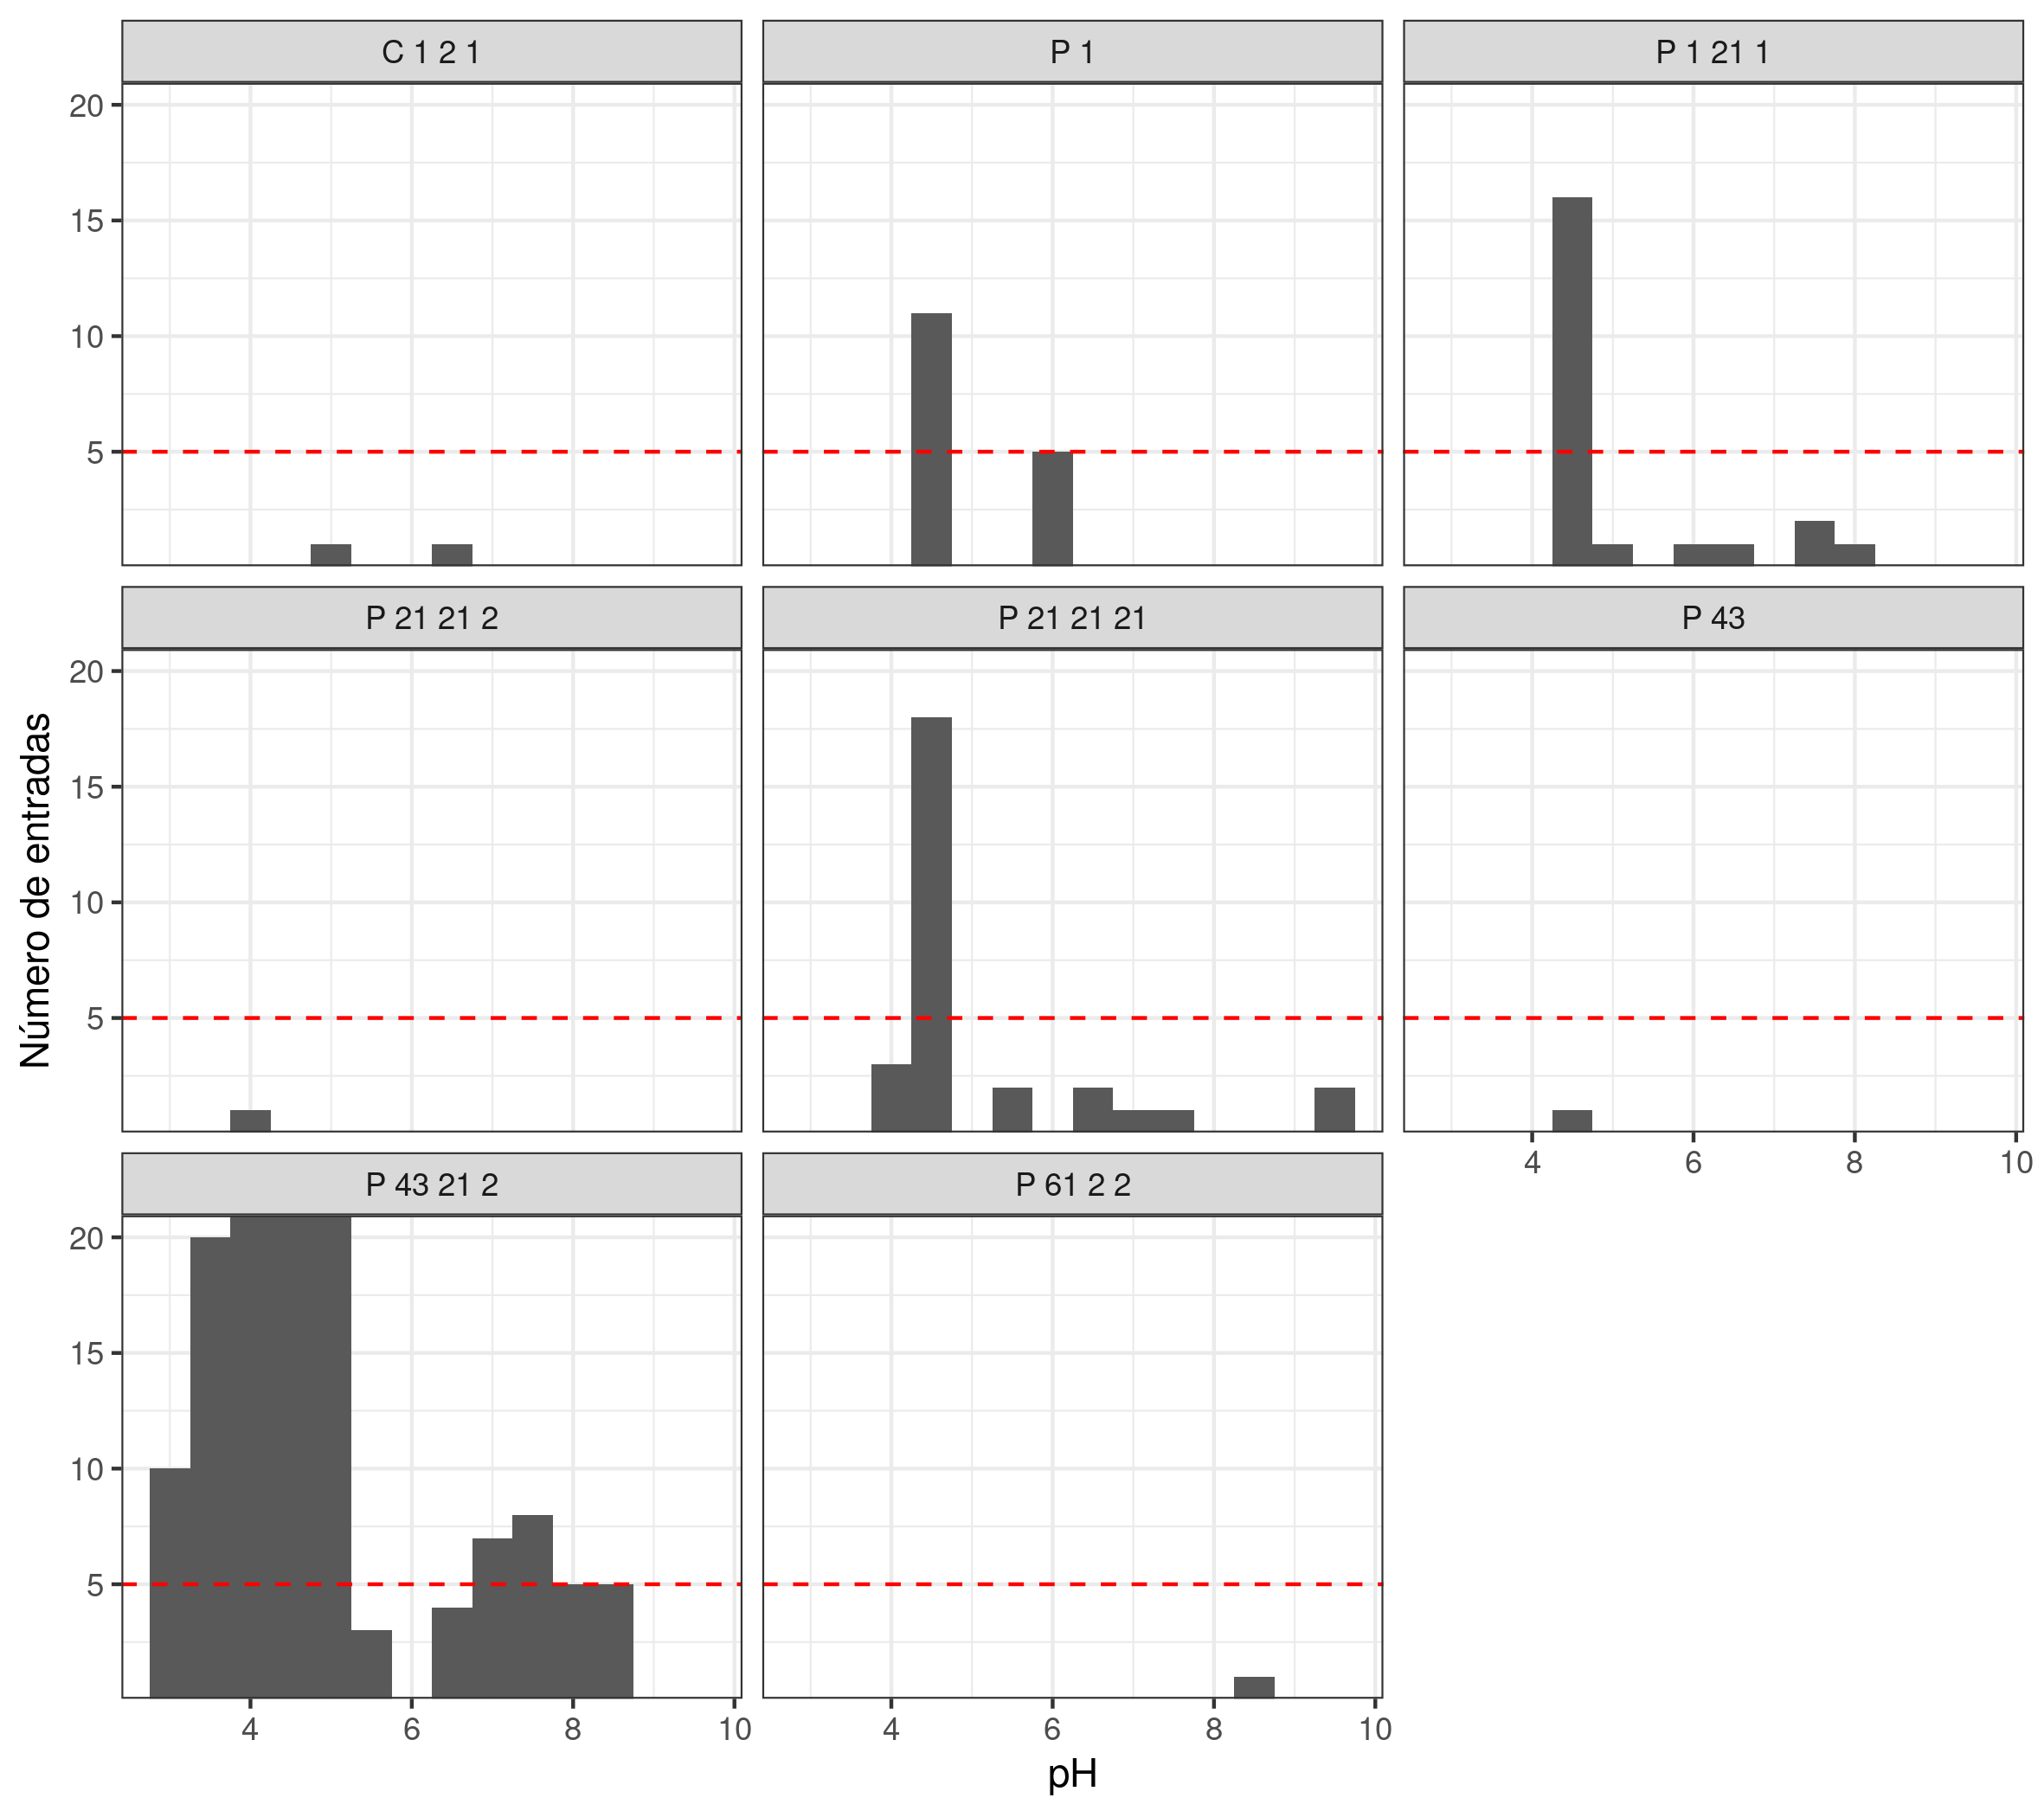
\includegraphics[width=0.8\textwidth]{imgs/hist_pH_by_gpo_P00698}
	\caption[Análisis visual]{Ejemplo del análisis visual: histograma de \texttt{P00698}. Nótese, en el gráfico de caja, que esta proteína tiene un amplio intervalo de pH $\sim~5$, en particular cuando cristaliza en el grupo espacial \texttt{P 43 21 2}. En este caso, la mayor parte de las estructuras están cristalizadas a un pH cercano a \num{4.7}, de ahí la forma final del gráfico de caja. Su frecuencia de cristalización en este mismo intervalo, según el histograma, es arriba de cinco (denotado por la línea horizontal roja), por lo  menos para buena parte del intervalo.}
	\labfig{fig:vis-anal}
\end{figure}


%\pagelayout{wide} % No margins
%\addpart{Apéndices}
%\pagelayout{margin} % Restore margins


%----------------------------------------------------------------------------------------

\backmatter % Denotes the end of the main document content
\setchapterstyle{plain} % Output plain chapters from this point onwards

%----------------------------------------------------------------------------------------
%	BIBLIOGRAPHY
%----------------------------------------------------------------------------------------

% The bibliography needs to be compiled with biber using your LaTeX editor, or on the command line with 'biber main' from the template directory

\defbibnote{bibnote}{Listado de referencias por orden de aparición.\par\bigskip} % Prepend this text to the bibliography
\printbibliography[heading=bibintoc, title=Referencias, prenote=bibnote] % Add the bibliography heading to the ToC, set the title of the bibliography and output the bibliography note

%\defbibnote{bibnote}{Here are the references in citation order.\par\bigskip} % Prepend this text to the bibliography
%\printbibliography[heading=bibintoc, title=Bibliography, prenote=bibnote] % Add the bibliography heading to the ToC, set the title of the bibliography and output the bibliography note

%----------------------------------------------------------------------------------------
%	INDEX
%----------------------------------------------------------------------------------------

% The index needs to be compiled on the command line with 'makeindex main' from the template directory

\printindex % Output the index

\end{document}
